\section{Mininet Setup} \label{sec:SDNNetSim}
The Mininet environment \cite{Mininet} has been used to emulate a SDN network to validate our methodology in terms of prediction accuracy and control performance. This software runs a collection of virtual network elements (i.e. end-hosts, switches, routers, and links) on a single Linux kernel using lightweight virtualization. 
%To test the effectiveness of the realized controller a simulated network has been programmed using the Mininet environment as a network emulation orchestration system. This software runs a collection of end-hosts, switches, routers, and links on a single Linux kernel by using lightweight virtualization to make a single system look like a complete network. Mininet's virtual objects emulate real SDN network devices. It is usually possible to create a Mininet network that resembles a hardware network, or a hardware network that resembles a Mininet network, and to run the same binary code and applications on either platform.
To generate traffic we used the D-ITG generator \cite{Avallone2004, Botta2012, Botta2013}.

\begin{figure}[tb!]
	\centering
	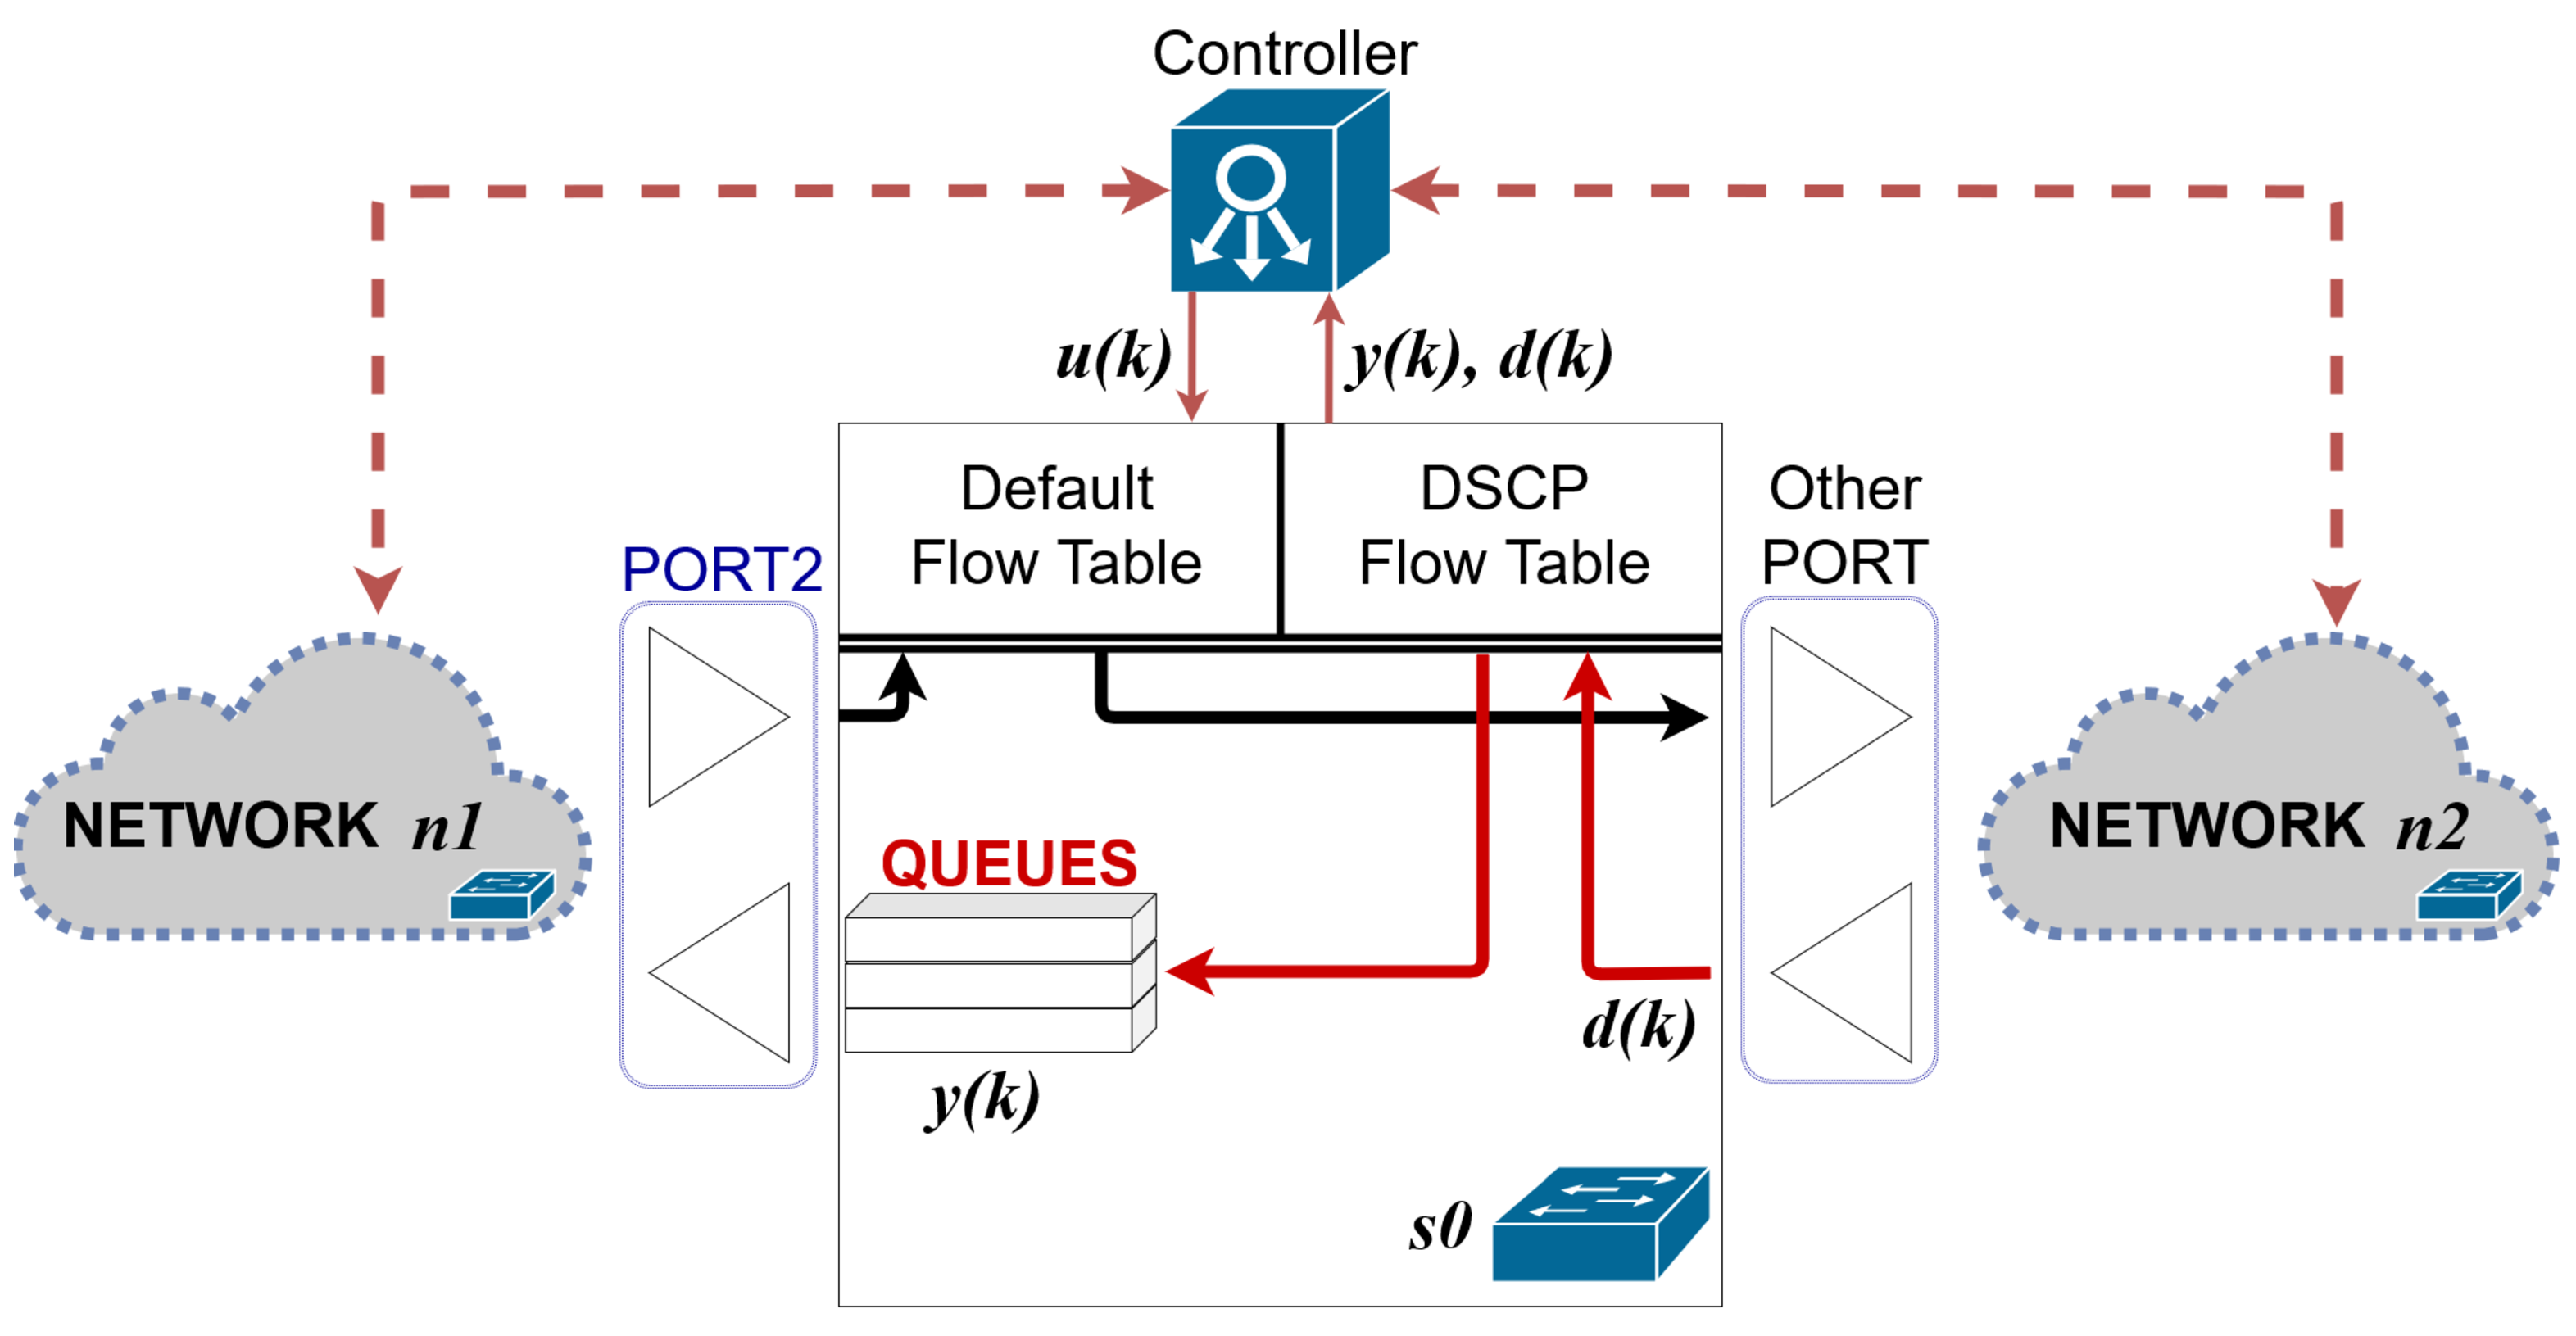
\includegraphics[keepaspectratio,width=\columnwidth]{figure/SDN_net_EPS.eps}
	\caption{Mininet emulated network architecture.}
	\label{fig:{Network}}
\end{figure}
%\begin{figure}[tb!]
%	\centering
%	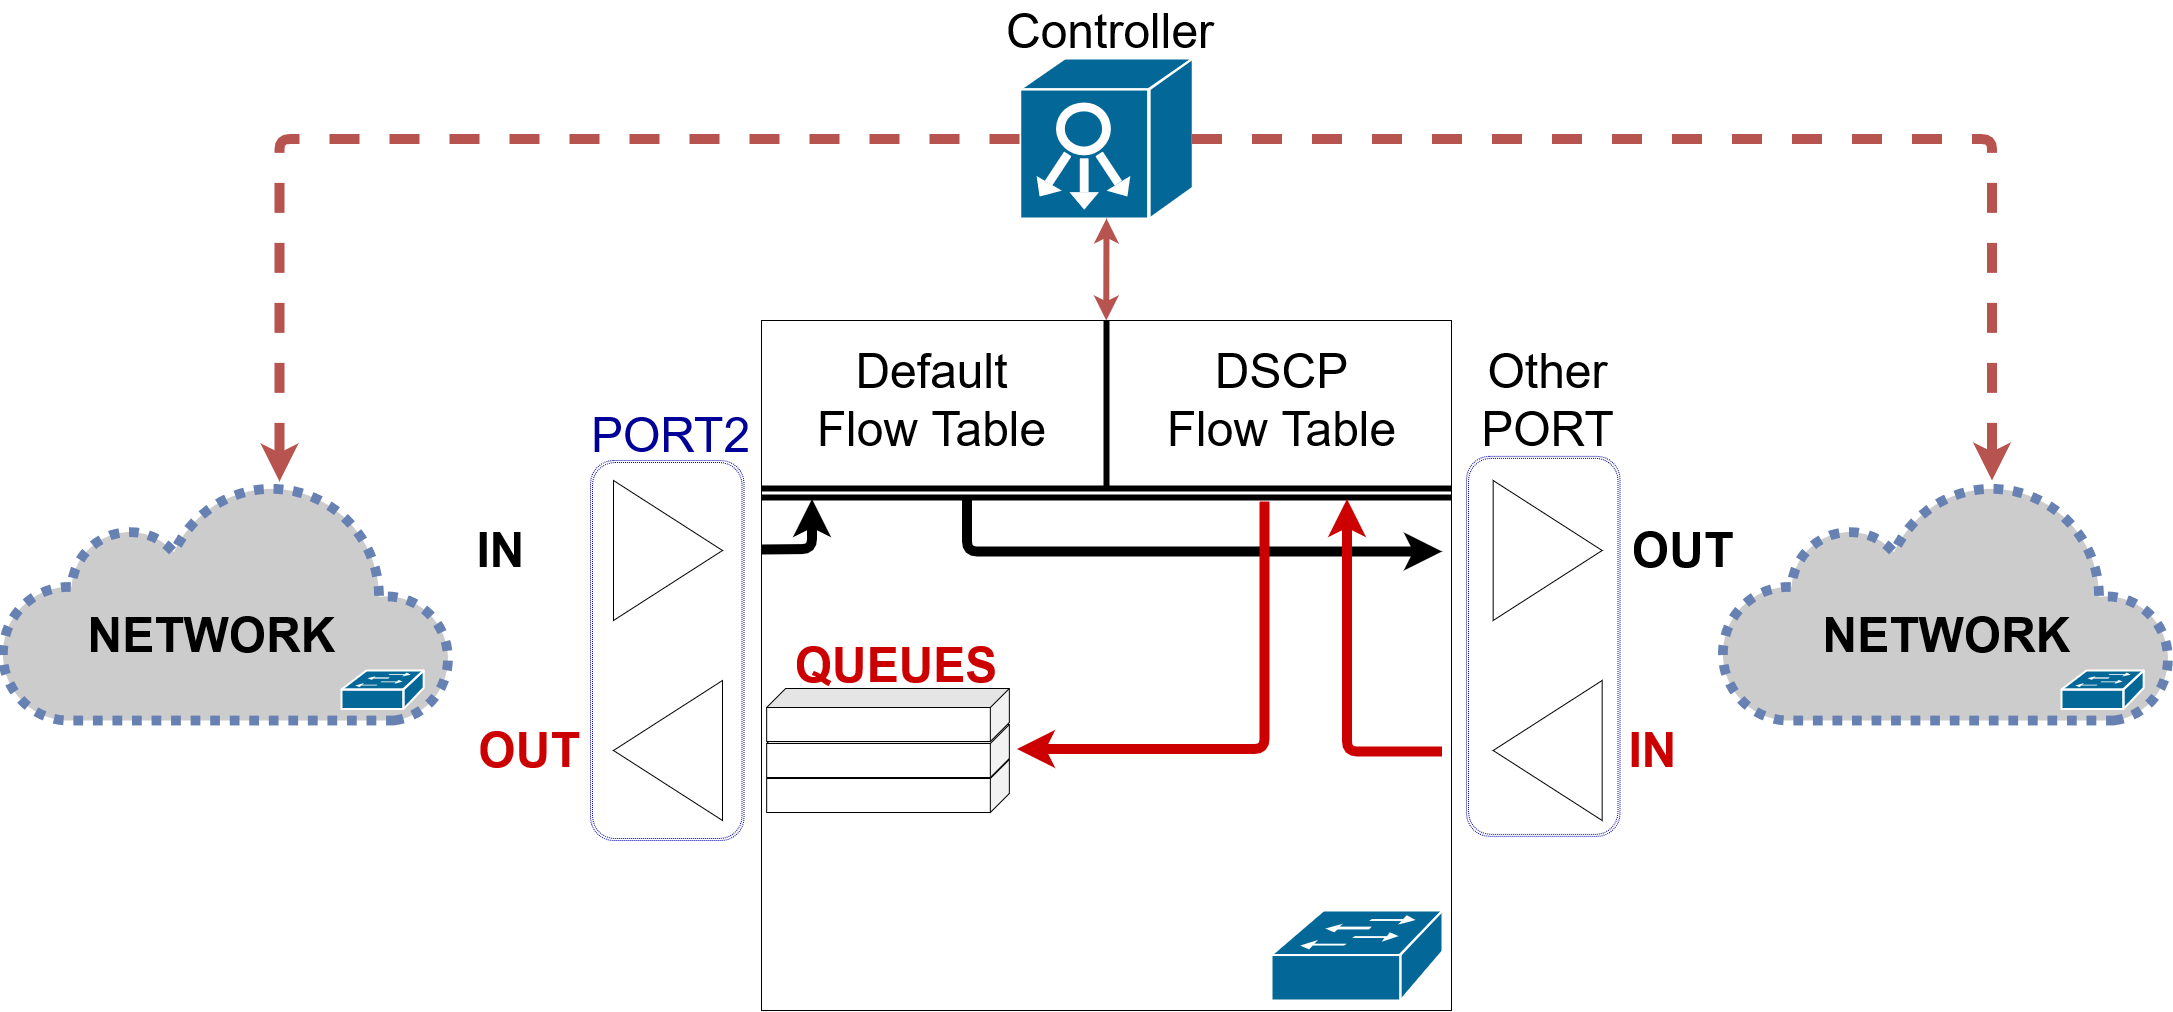
\includegraphics[width=13cm]{figure/SDN_net_LAST.png}
%	\caption{Simulated Network inside Mininet environment.}
%	\label{fig:{Network}}
%\end{figure}

We consider a network architecture as in Figure \ref{fig:{Network}}, which aims at representing a portion of a larger network where a bottleneck occurs. More precisely, we consider a switch $s0$ with one input port and one output port, and a remote controller \cite{OVS, RYU} that dynamically manages the configuration of the queues of $s0$. The input of $s0$ is fed with an instance of D-ITG generating stochastic traffic, whose mean value follows the pattern of a real data set (where packets are differentiated by their ToS - Type of Service - priority index) extracted from two days logs of a router of a large service provider network. Namely, the original real data set contains traffic of a real network incoming from a source geographic area and terminating in a destination geographic area, and is divided for each value of Differentiated Services Code Point (DSCP) with a sampling time of 5 minutes \cite{Baker1998, Babiarz2006}. We recall that DSCP is the modern definition of the Type of Service (ToS) field, in which the first 6 bits are the Differentiated Services field that are in common with ToS field, and the last 2 bits regard explicit congestion notification. The ToS field can specify the priority of a datagram and the request for a low delay addressing, a high throughput or a high reliability service. Following the implementation of many national service provider networks (see e.g. \cite{Notiziario}), we partition the 8 different values of the DSCP in three classes: the \textit{Default} class (DSCPs $0,1,3$), the \textit{Premium} (DSCPs $2,4,6,7$), and the \textit{Gold} class (DSCP $5$): to each class we will assign a single queue, associated with a different priority.

%Traffic generation is entrusted to the D-ITG generator which uses informations inside a database created from a real measure that contains the number of packets transmitted and received by a switch. The database fields has been divided for each type of Differentiated Services Code Point (DSCP) with a sampling time of 5 minutes \cite{Baker1998, Babiarz2006}. DSCP is the modern definition of the Type of Service (ToS) field in which the first 6 bits are the Differentiated Services field that are in common with ToS field, and the last 2 bits are the explicit congestion notification. The ToS field can specify the priority of a datagram and the request for a low delay addressing, a high throughput or a high reliability service. Depending on the ToS values, a packet could be placed in a high priority exit queue, or follow a route with latency, throughput and the appropriate reliability for the request.


Using D-ITG Sender and Receiver SW modules it has been possible to establish a connection between networks n1 and n2. In particular, 16 ITG modules have been initialized: 8 for each network, and within each network one for each DSCP index. These modules handle the sampling time interval (5 minutes), the inter-departure time stochastic distribution associated with the packet rate, the packet size stochastic distribution, the IP and port destinations, and the DSCP index. Regarding the controller SW module we used Ryu, which provides software components with well defined Application Programming Interfaces (API) that give the possibility to easily create new network management and control applications. Ryu supports various protocols for managing network devices, such as OpenFlow, Netconf, OF-config, etc. About OpenFlow, Ryu supports fully 1.0, 1.2, 1.3, 1.4, 1.5 and Nicira Extensions. For our test-bed the 1.3 version has been chosen. In particular, APIs were used for queue control and counter recovery from the switches \cite{ofctlrest,QoS}. The feedback information collected for the purposes of this work are the descriptions of switches, ports and queues, the number of packets received and transmitted on each port of a switch, the packets passing through the flow tables, the packet rate values of each queue and the packets transmitted by each single queue. In summary, the variables associated to the traffic and control signals in our closed-loop architecture are as follows:

\begin{itemize}
	\item $d(k)\in\Real^{10}$ is a measurable disturbance vector, i.e. representing variables we cannot control. The first 8 components $d_1(k),\ldots,d_8(k)$ consist of the number of packets incoming in the switch $s0$ differentiated with respect to the 8 different values of the DSCPs. $d_9(k)$ and $d_{10}(k)$ are proxy variables, i.e. the hours and minutes of the day, which are very useful to the predictive model since traffic dynamics are tightly correlated with them, e.g. they are substantially different between night and day;
	\item $y(k)\in\Real^{3}$ is the measured output vector, i.e. the variables we want to regulate. They consist of the number of packets outgoing from switch $s0$ differentiated with respect to the corresponding service class: $y_1(k)$ is the Default Queue output, $y_2(k)$ is the Premium Queue output and $y_3(k)$ is the Gold Queue output;
	\item $u(k)\in\Real^{3}$ is the control input vector. Each component corresponds to the queue configuration of each service class: $u_1(k)$ is the Default Queue configuration, i.e. the maximum admitted bandwidth; $u_2(k)$ is the Premium Queue configuration, i.e. the maximum admitted bandwidth; $u_3(k)$ is the Gold Queue configuration, i.e. the minimum admitted bandwidth;
\end{itemize}

\begin{figure}[tb!]
	\centering
	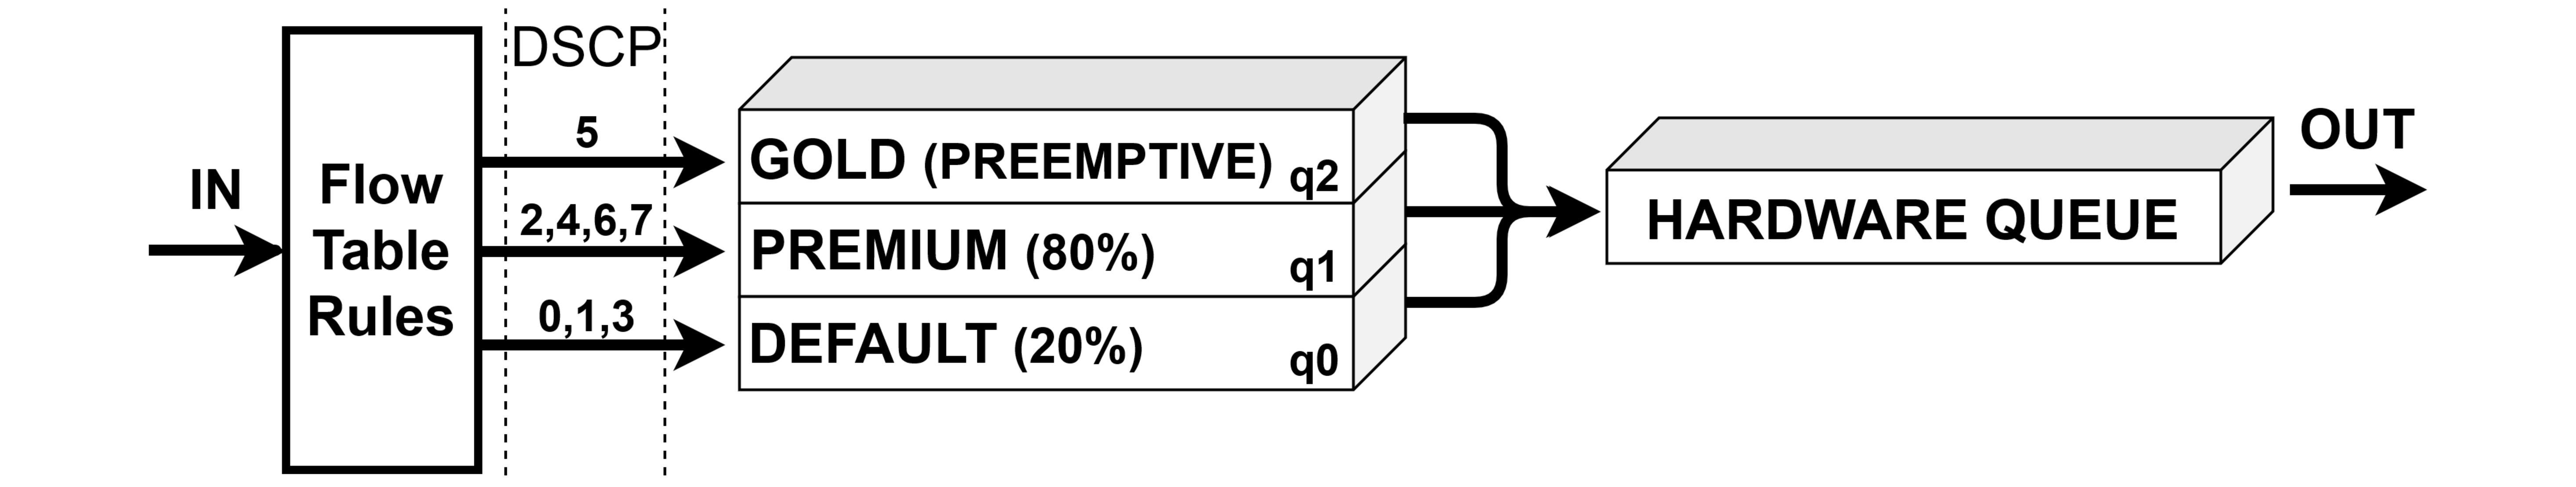
\includegraphics[keepaspectratio,width=\columnwidth]{figure/QUEUE.eps}
%	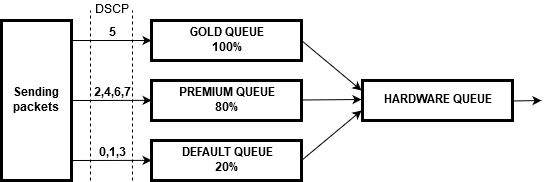
\includegraphics[keepaspectratio,width=12cm]{figure/queue.png}
	\caption{Static queues rate with routed packets relative to DSCP.}
	\label{fig:{queue}}
\end{figure}

In this work we first applied in our emulative scenario the static control of queues used in the Italian service provider network of \textit{Telecom Italia} \cite{Notiziario}, which is depicted in Figure \ref{fig:{queue}}. To this aim we defined 3 queues in $s0$ and configured the queues as follows: packets with the DSCP values 0, 1 and 3 (Default queue) are routed via queue 0, with maximum rate $u_1(k) = 20 \textit{MB/s}, \forall k$; the packets with values 2, 4, 6 and 7 (Premium queue) are routed on queue 1, with maximum rate $u_2(k) = 80 \textit{MB/s}, \forall k$; the packets with value 5 (Gold queue) are routed on queue 2, with minimum rate $u_3(k) = 100 \textit{MB/s}, \forall k$. To obtain this prioritization it has also been necessary to set the flow tables of $s0$ to discriminate incoming packets based on the DSCP value and the destination IP address, and re-route them to the desired queue. Also, to obtain a bottleneck situation in $s0$, we have chosen the bandwidth of the output port of switch $s0$ at 100 \textit{MB/s}. Using this configuration queue 2 uses the maximum capacity of the port to forward packets with preemptive priority, while the other two queues use the remaining bandwidth from 0 \textit{MB/s} to the specified maximum bandwidth based on needs.
%As formally defined later in Section \ref{secSwitchedModeling}, the packets sent by the queues will be collected in the state vector to be controlled $x(k)\in\mathbf{R}^3,\ \forall k$,  while the bandwidth associated to the queues will compose the control variables vector $u(k)\in\mathbf{R}^3,\ \forall k$.

As we will see in Section \ref{secExpRes}, using static priority control the queues will not be able to send all the packets incoming from network $n1$, and a dramatic amount of packets will be lost. This motivates the application of optimization techniques, which are enabled by the predictive models derived using the methodology described in the following section.

\section{Simulation results}\label{secExpRes}
In this section simulation results of the application of the proposed approach to SDN Priority Queueing identification and control will be provided. Standard RFs are used to derive predictive models of the disturbance components $d_1(k),\ldots,d_8(k)$, i.e. the switch input differentiated for each DSCP index, and validate the accuracy. Then the validation of accuracy of the predictive model of the output variable $y(k)$ derived as illustrated in Section \ref{secSwitchedModeling} is shown: the predictive models (based on RTs and RFs) will be compared with Artificial Neural Networks, showing that RFs represent the ideal solution both in terms of prediction accuracy and computational complexity; then it will be illustrated the effect of iterative dataset updates in the prediction accuracy, both with and without prediction of the future disturbances. Finally it will be used the proposed predictive models to setup a MPC problem (see Problem \ref{pbMPC}), and validate the control performance in terms of packet losses reduction and bandwidth saving, both with and without prediction of the future disturbances. It will also be shown, as expected, that using accurate predictive models and applying MPC provides dramatic reduction of packet losses and increase of bandwidth saving with respect to the static bandwidth allocation policy used in Service Provider Networks as described in Section \ref{sec:SDNNetSim}: even thought this result is not surprising, it is decided to quantify the gap to emphasize that much better performance can be obtained in real networks just collecting historical data and applying a controller that can be directly implemented using the accurate models of the proposed identification algorithm and Quadratic Programming solvers (which are well known to be very efficient).

In each of the aforementioned validations, 4 different predictive models have been exploited, using iteratively enriched data sets. More precisely, \textbf{OLD} is a predictive model identified with a data set of $5124$ samples, collected with a sampling time of $5$ minutes and obtained from network emulation with random values of the input $u(k)$; \textbf{1UP} is a predictive model identified with the \textbf{OLD} data set enriched with $3456$ new samples obtained from network emulation when applying closed-loop MPC to define the input $u(k)$; \textbf{2UP} is a predictive model identified with the \textbf{1UP} data set enriched with $3168$ new samples obtained from network emulation when applying closed-loop MPC to define the input $u(k)$; \textbf{3UP} is a predictive model identified with the \textbf{2UP} data set enriched with $6336$ new samples obtained from network emulation when applying closed-loop MPC to define the input $u(k)$. An independent data-set composed by $1684$ samples is used to validate the above models.
%Before running the identification algorithms, the dataset has been pre-processed checking if all measurements were coherent and if there were voids or data misalignments that could have distorted the model.
All simulations have been ran on a UDOO x86 Advanced with an Intel Braswell N3160 processor up to 2.24 GHz and 4 GB of RAM \cite{UDOO}.

\subsection {Disturbance predictive model validation} Having an accurate model of the variable $d(k)$ (i.e. the switch input differentiated for each DSCP index) can be helpful to improve the model identification performance as well as the reference input $x_\mathrm{ref}$ to follow in Problem \ref{pbMPC}. In this section we apply standard RF algorithms, with a regressive index of $15$ steps and $30$ trees for each forest, to obtain a predictive model of the disturbance over a predictive horizon of $N=5$ ($25$ minutes): this choice of $N$ has been taken considering the tradeoff between time complexity of the identification algorithm and the obtained identification accuracy. 

\begin{figure}[h!]
	\centering
	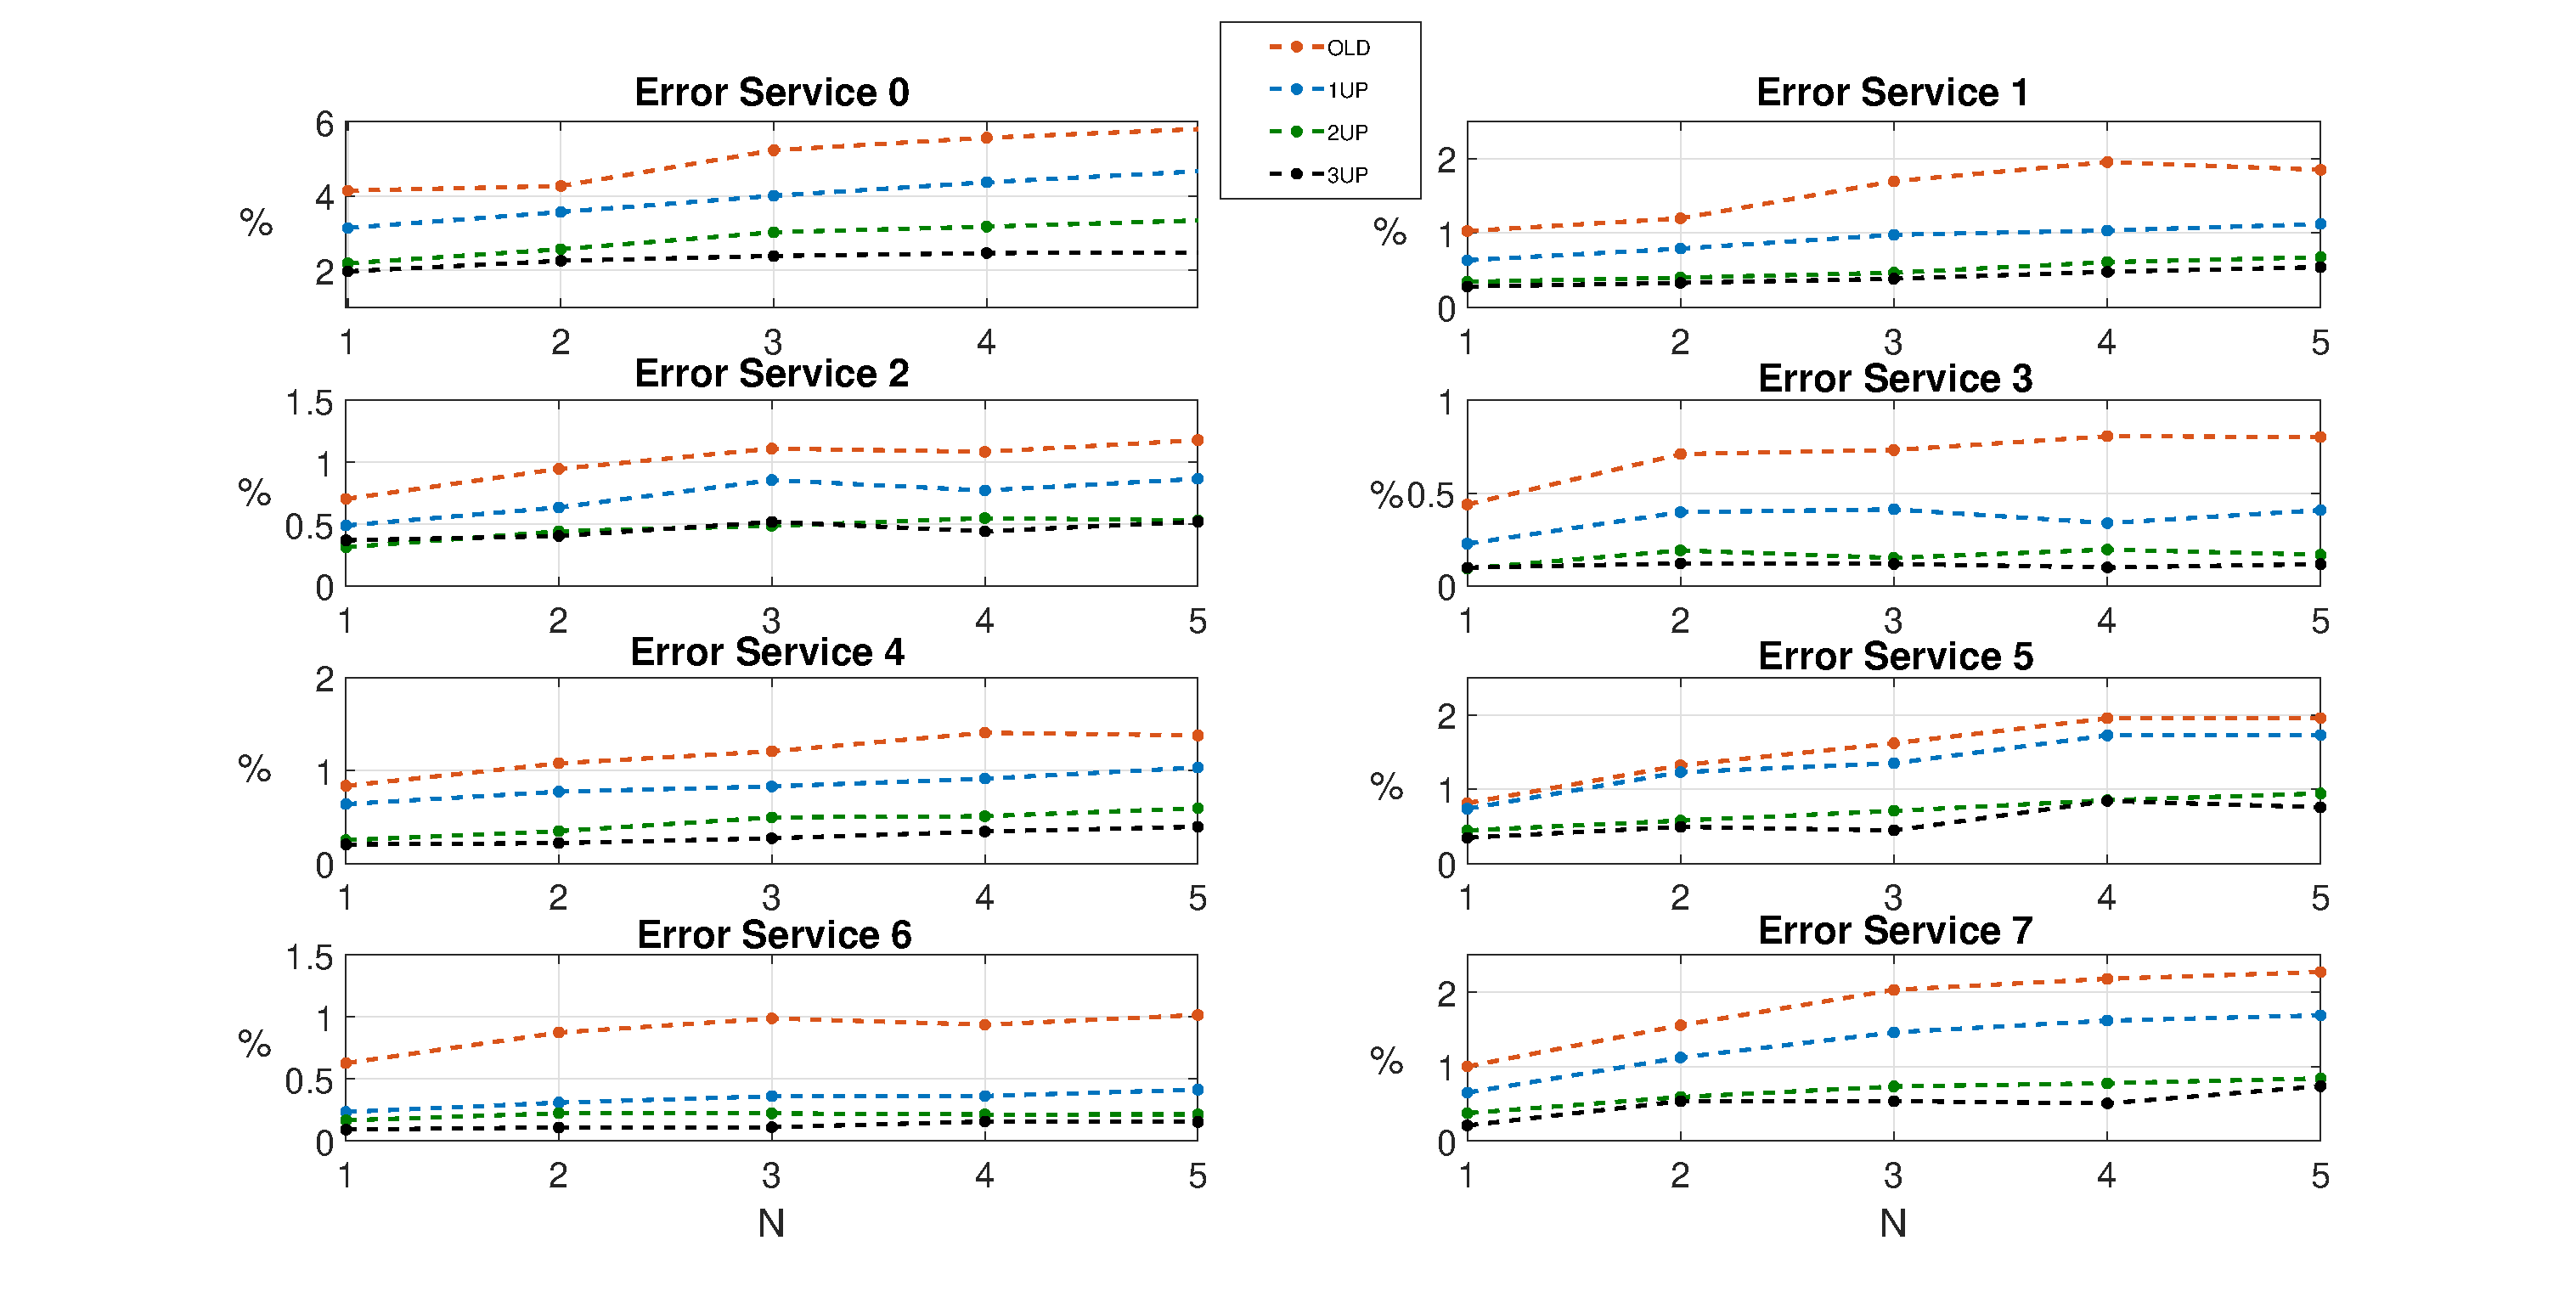
\includegraphics[trim={120 0 120 0}, width=1\linewidth]{figure/Error_Disturbance.eps}
	\caption{NRMSE of the disturbance predictive model over a time horizon of $N=5$.}
	\label{fig:{errorDist}}
\end{figure}
\begin{figure}[h!]
	\centering
	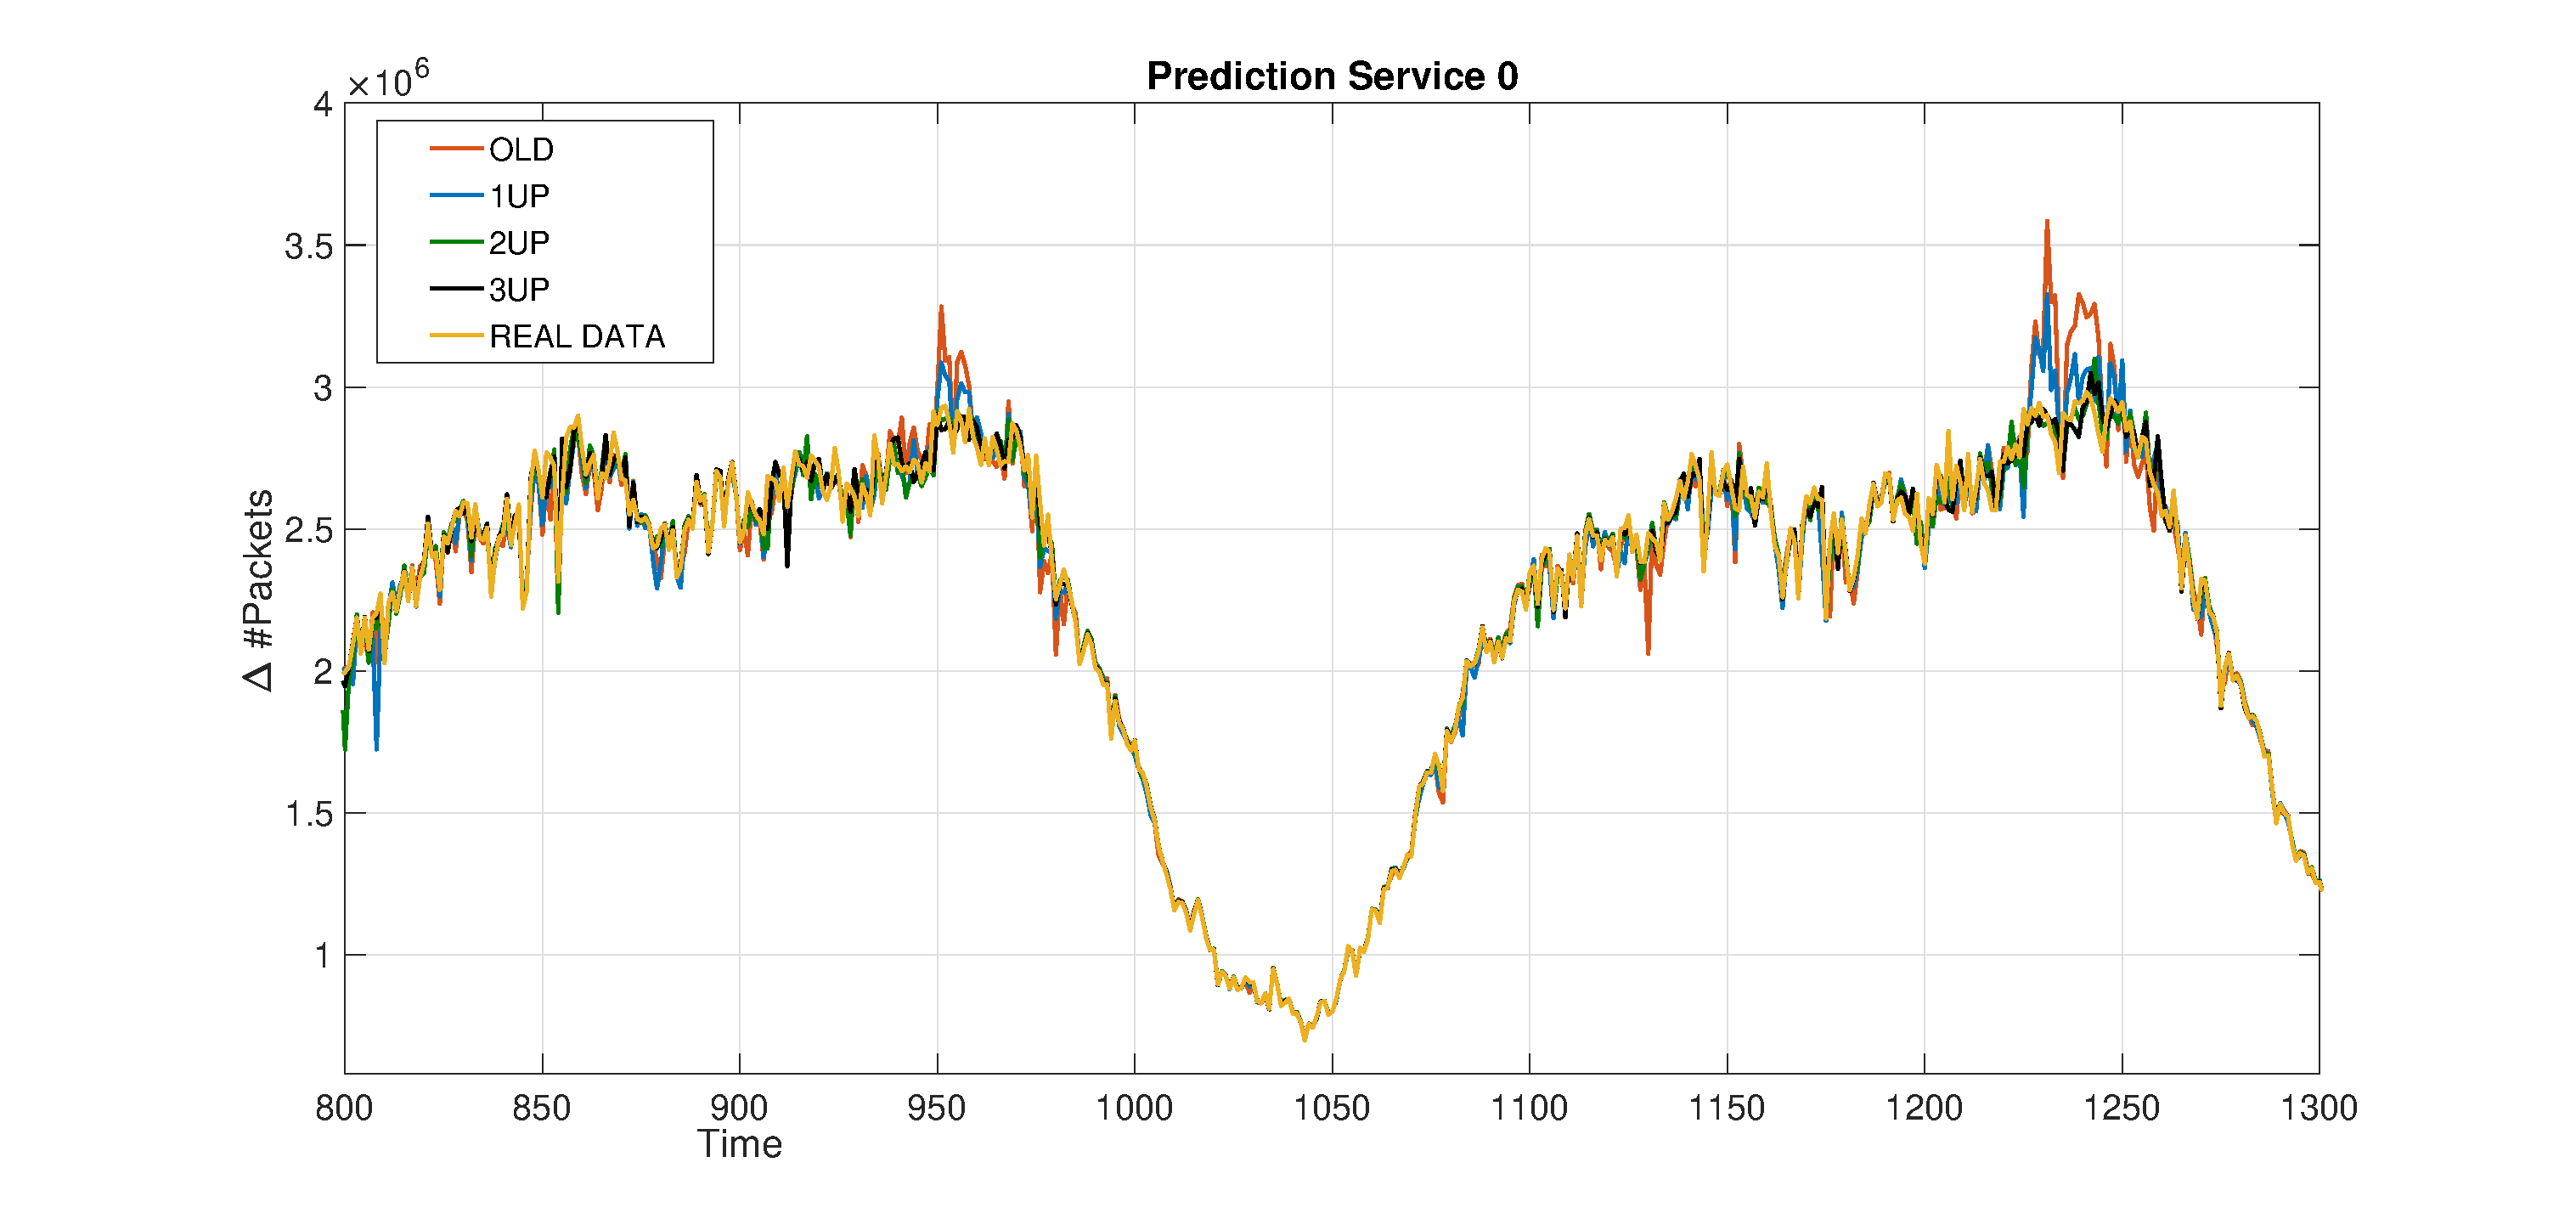
\includegraphics[trim={120 0 120 0}, width=1\linewidth]{figure/Error_Disturbance_Packets.eps}
	\caption{Comparison between the real traffic (YELLOW LINE) and the traffic prediction for the different models for Service 0.}
	\label{fig:{errorPack}}
\end{figure}

Figure \ref{fig:{errorDist}} shows the Normalised Root Mean Square Error (NRMSE) of the predictive model of the disturbance signals (one for each of the 8 DSCP indices) over a time horizon of $N=5$: the prediction error is worse for Service $0$ ($4-6\%$) since it includes the majority of the packets that transit through the switch. For other services the NRMSE is at most $2.2\%$ (Service 7) over all the predictive horizons. The improvement of the model accuracy when using larger (updated) data sets is evident, until a \textit{saturation} is reached and further data do not help to improve the model accuracy: the NRMSE significantly reduces and for Service 0 it is even halved. Figure \ref{fig:{errorPack}} plots, for Service $0$ and in a time window of $500$ samples (almost two days), the predictions of OLD, 1UP, 2UP and 3UP as well as the original data, and clearly highlights the better prediction of 2UP and 3UP with respect to OLD and 1UP.

%====================================================================================================

\subsection{Queues predictive model validation}

In this section we first compare the accuracy of our predictive models with Artificial Neural Networks. We recall that a neural network is a collection of algorithms that aim to identify underlying relations in a dataset: it consists of groups of connected neurons organized in layers, where the connections between neurons are modeled using weights. The signal produced with this linear composition is then fed into an activation function that is in general nonlinear. The reader is referred to \cite{NNstateOfART} and references therein for more details. A wide number of tools to build Neural Networks have been developed during recent years, e.g. \cite{tensorflow2015,chollet2015keras,openNN} just to mention a few: in this work we exploit the Deep Learning Toolbox of Matlab to compare predictive models based on NNs with the methodology proposed in this paper, based on ARX combined RTs and RFs. We consider here just OLD as the learning dataset and chose a predictive horizon $N=5$.

To identify a RT (resp. RF) based predictive model of the queues we trained a Regression Tree (resp. a Random Forest) for each output and for each time horizon, with a total of $15$ trees (resp. $15$ forests each consisting of $30$ trees). The main parameters used for the identification algorithm (see Section \ref{secSwitchedModeling} and Problem \ref{pbLeastSquareProblem}) are summarized in Table \ref{tab:idPar}.  
\begin{table}[h!]
	\caption{Identification parameters}
	\centering
	\begin{tabular}{c c c c}
		\hline\hline
		Parameters & Value & Parameters & Values\\ 
		\hline
		N               & 5    & $f_{min}$   &-100 \\
		$\nu$        & 1     & $f_{max}$  &100  \\
		$\delta_x$ & 5     & $a_{min}$  &-100  \\
		$\delta_u$ & 5     & $a_{max}$ &100 \\
		$\delta_d$ & 5   & $b_{min}$  &0  \\
		Minleaf      & 13   & $b_{max}$ &10000  \\
		$|\Fij|$      & 30  &                   &\\
		\hline
	\end{tabular}
	\label{tab:idPar}
\end{table}
In particular, the regressive terms ($\delta_d$, $\delta_x$, $\delta_u$) and the minimum number of samples for each tree of each forest (MinLeaf) have been chosen, with a trial and error approach, considering that very small regressive horizons and very large values for MinLeaf may lead to inaccurate prediction (as they do not provide sufficient information on the past) but very large regressive horizons and very small values for MinLeaf also lead to inaccurate prediction (as they interpolate very old data that might negatively affect the results and produce overfitting).

Regarding specific parameters used for running NN, and for the sake of a fair comparison, we tuned them to obtain the best performance: in particular we considered shallow networks of 2 layers since depper networks did not improve the accuracy and, instead, have the negative effect of increasing the sensitivity of the accuracy with respect to the initial conditions of the weights. Among the many algorithms for optimizing the weights of the neurons we exploited the \textit{Scaled conjugate gradient back-propagation} described in \cite{Moller1990}, which provided the best accuracy with respect to our dataset. Regarding the activation functions, we used both the classical sigmoid function (\textit{LogSig}) and the Hyperbolic tangent sigmoid transfer function (\textit{TanSig}).
\begin{figure}[h!]
	\centering
	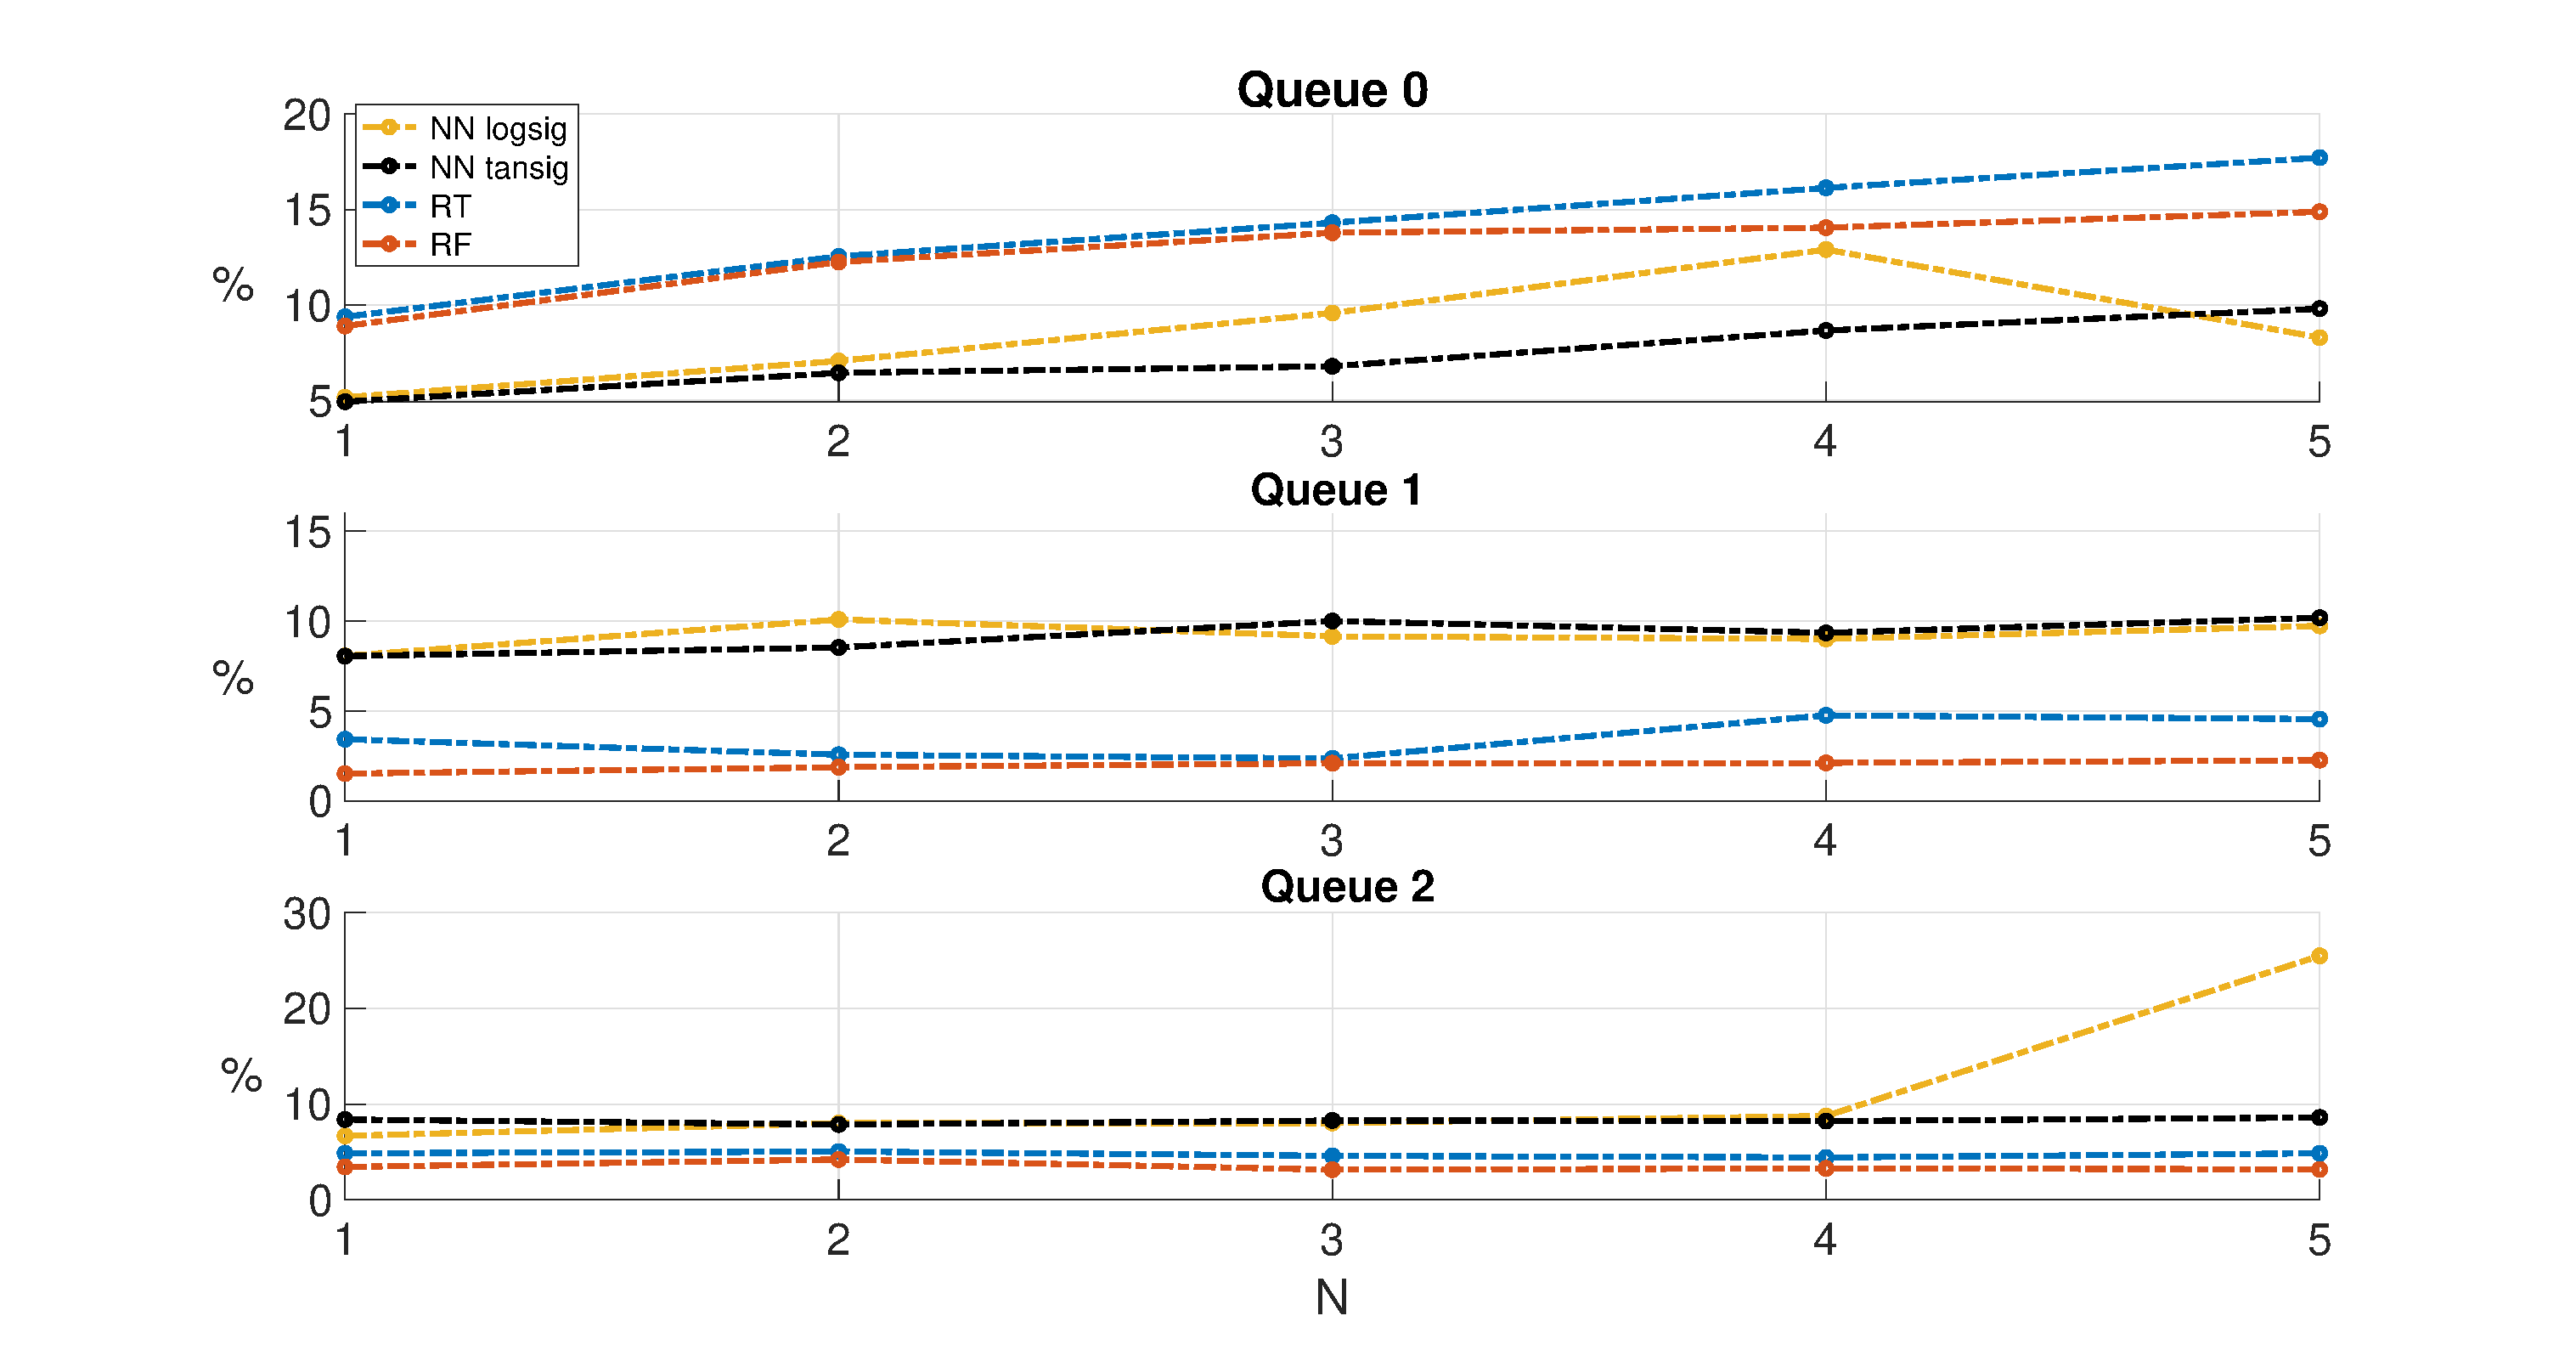
\includegraphics[trim={120 0 120 0},width=0.9\linewidth]{figure/NRMSENNvsRTvsRF.eps}
	\vspace{-0.2cm}
	\caption{NRMSE, up to $N=5$ and for each priority class, for RT (blue), RF (red), NN with sigmoids as activation function (yellow) and NN with hyperbolic tangent as activation function (black).}
	\label{fig:{NRMSE}}
\end{figure}

As a metric of the prediction accuracy we compared in Figure \ref{fig:{NRMSE}} the Normalized Root Mean Square Errors (NRMSE) of the different identification approaches for each priority class and over a horizon up to $N=5$. Regarding queue $0$ (Default) NNs perform better than RT and RF, but in queues $1$ (Premium) and $2$ (Gold), characterised by higher priority, RF provides the best performance. Queue $0$ is characterised by a larger NRMSE with all identification techniques: this is due to the fact that, having the lowest priority, it suffers more packet losses and this can negatively affect the prediction accuracy. Our validation emphasizes that RTs, even thought very simple and fast to compute, are often affected by overfitting and variance issues, i.e. small variations of the training data result in large variations of the tree structure and, consequently, of the predictions. Regarding NNs, they provide a less accurate model in 2 cases over 3. Indeed, by analyzing the dataset distribution, we noticed a peculiar regular grid pattern that can be very well approximated by hyper-rectangles: since RTs and RFs base their prediction on hyper-rectangular dataset partitions, the better performance with respect to NNs is reasonable. For queue 0, even thought NNs perform better, we need to remark that their predictive model is based on nonlinear functions: this makes the derived model impractical for real-time control as the corresponding MPC formulation turns into a nonlinear optimization problem, for which there is no approach that can guarantee neither a global optimal solution nor a reasonable computation time. In addition to this, even obtaining a closed mathematical form of the predictive function of a Neural Network starting from neurons and weitghts is not always an easy task, because of the highly nonlinear interconnections between the different layers. For all these reasons we decided to only use from now on RF-based models, which provide the best choice both from the accuracy and the computational complexity points of view. In the following we illustrate the effect of iterative dataset updates in the prediction accuracy, both with and without knowledge of the future disturbances.
\begin{figure}[th!]
	\centering
	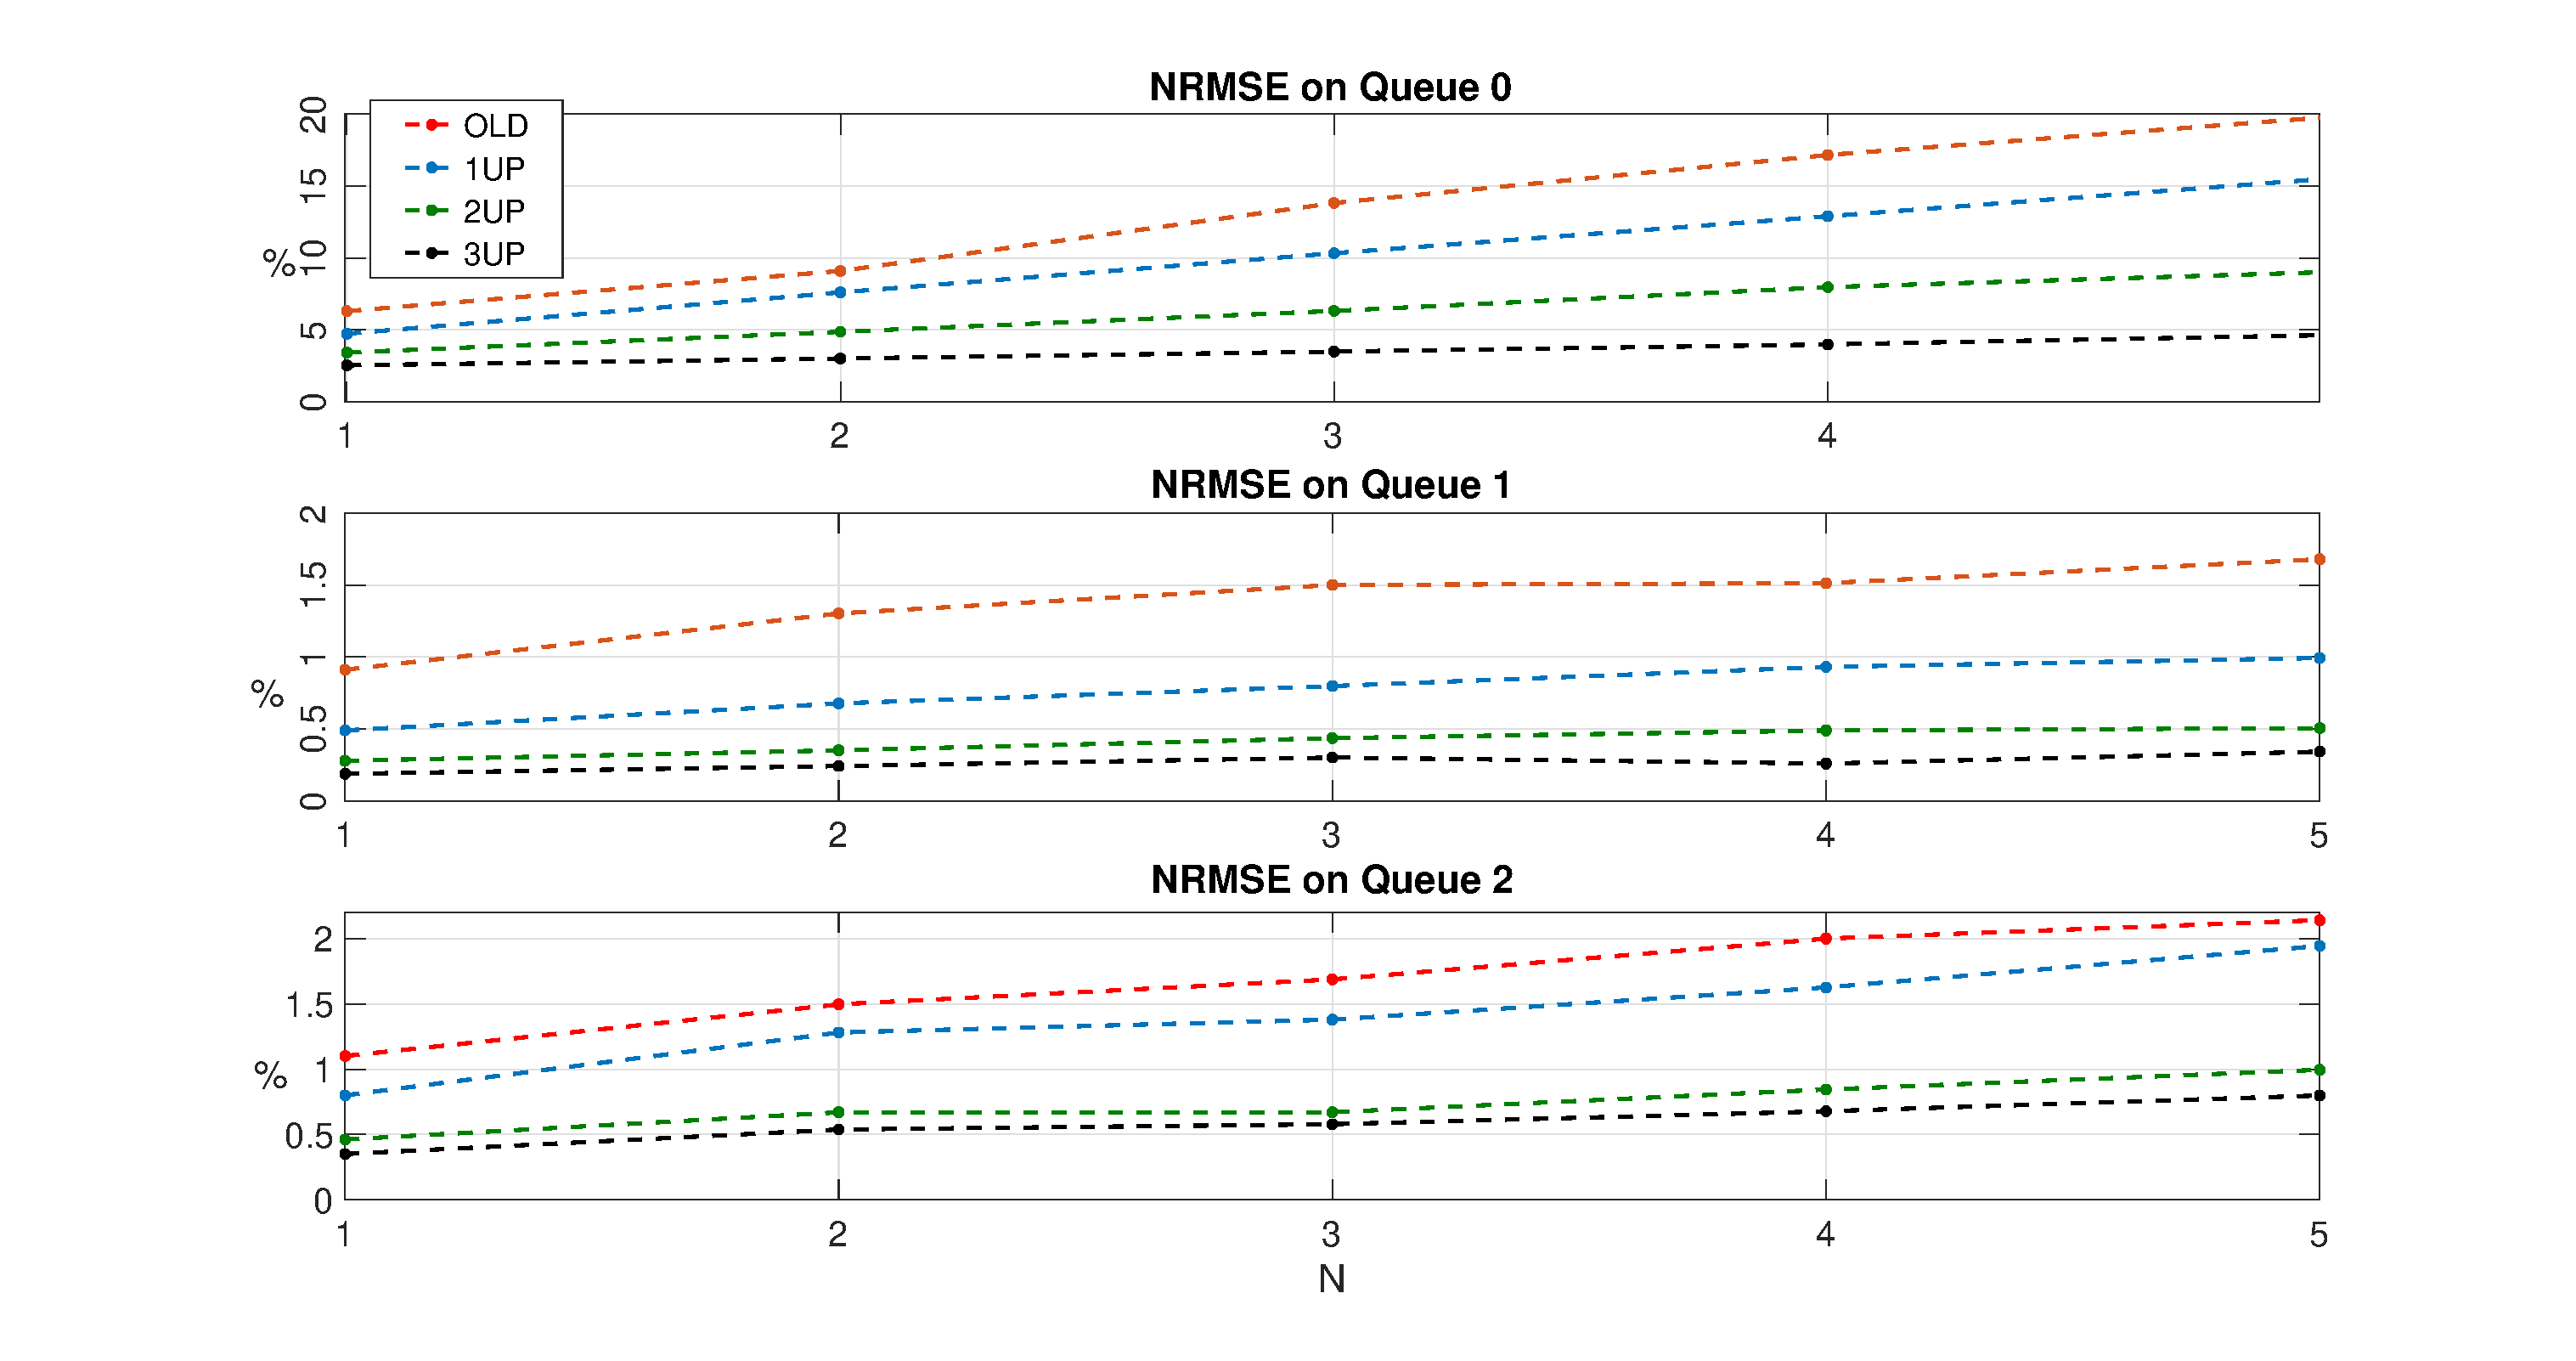
\includegraphics[trim={120 0 120 0}, width=0.9\linewidth]{figure/Error_State.eps}
	\caption{NRMSE of the queues output predictive model over a time horizon of $N=5$, without knowledge of the future disturbances}
	\label{fig:{stateNRMSE}}
\end{figure}
\begin{figure}[th!]
	\centering
	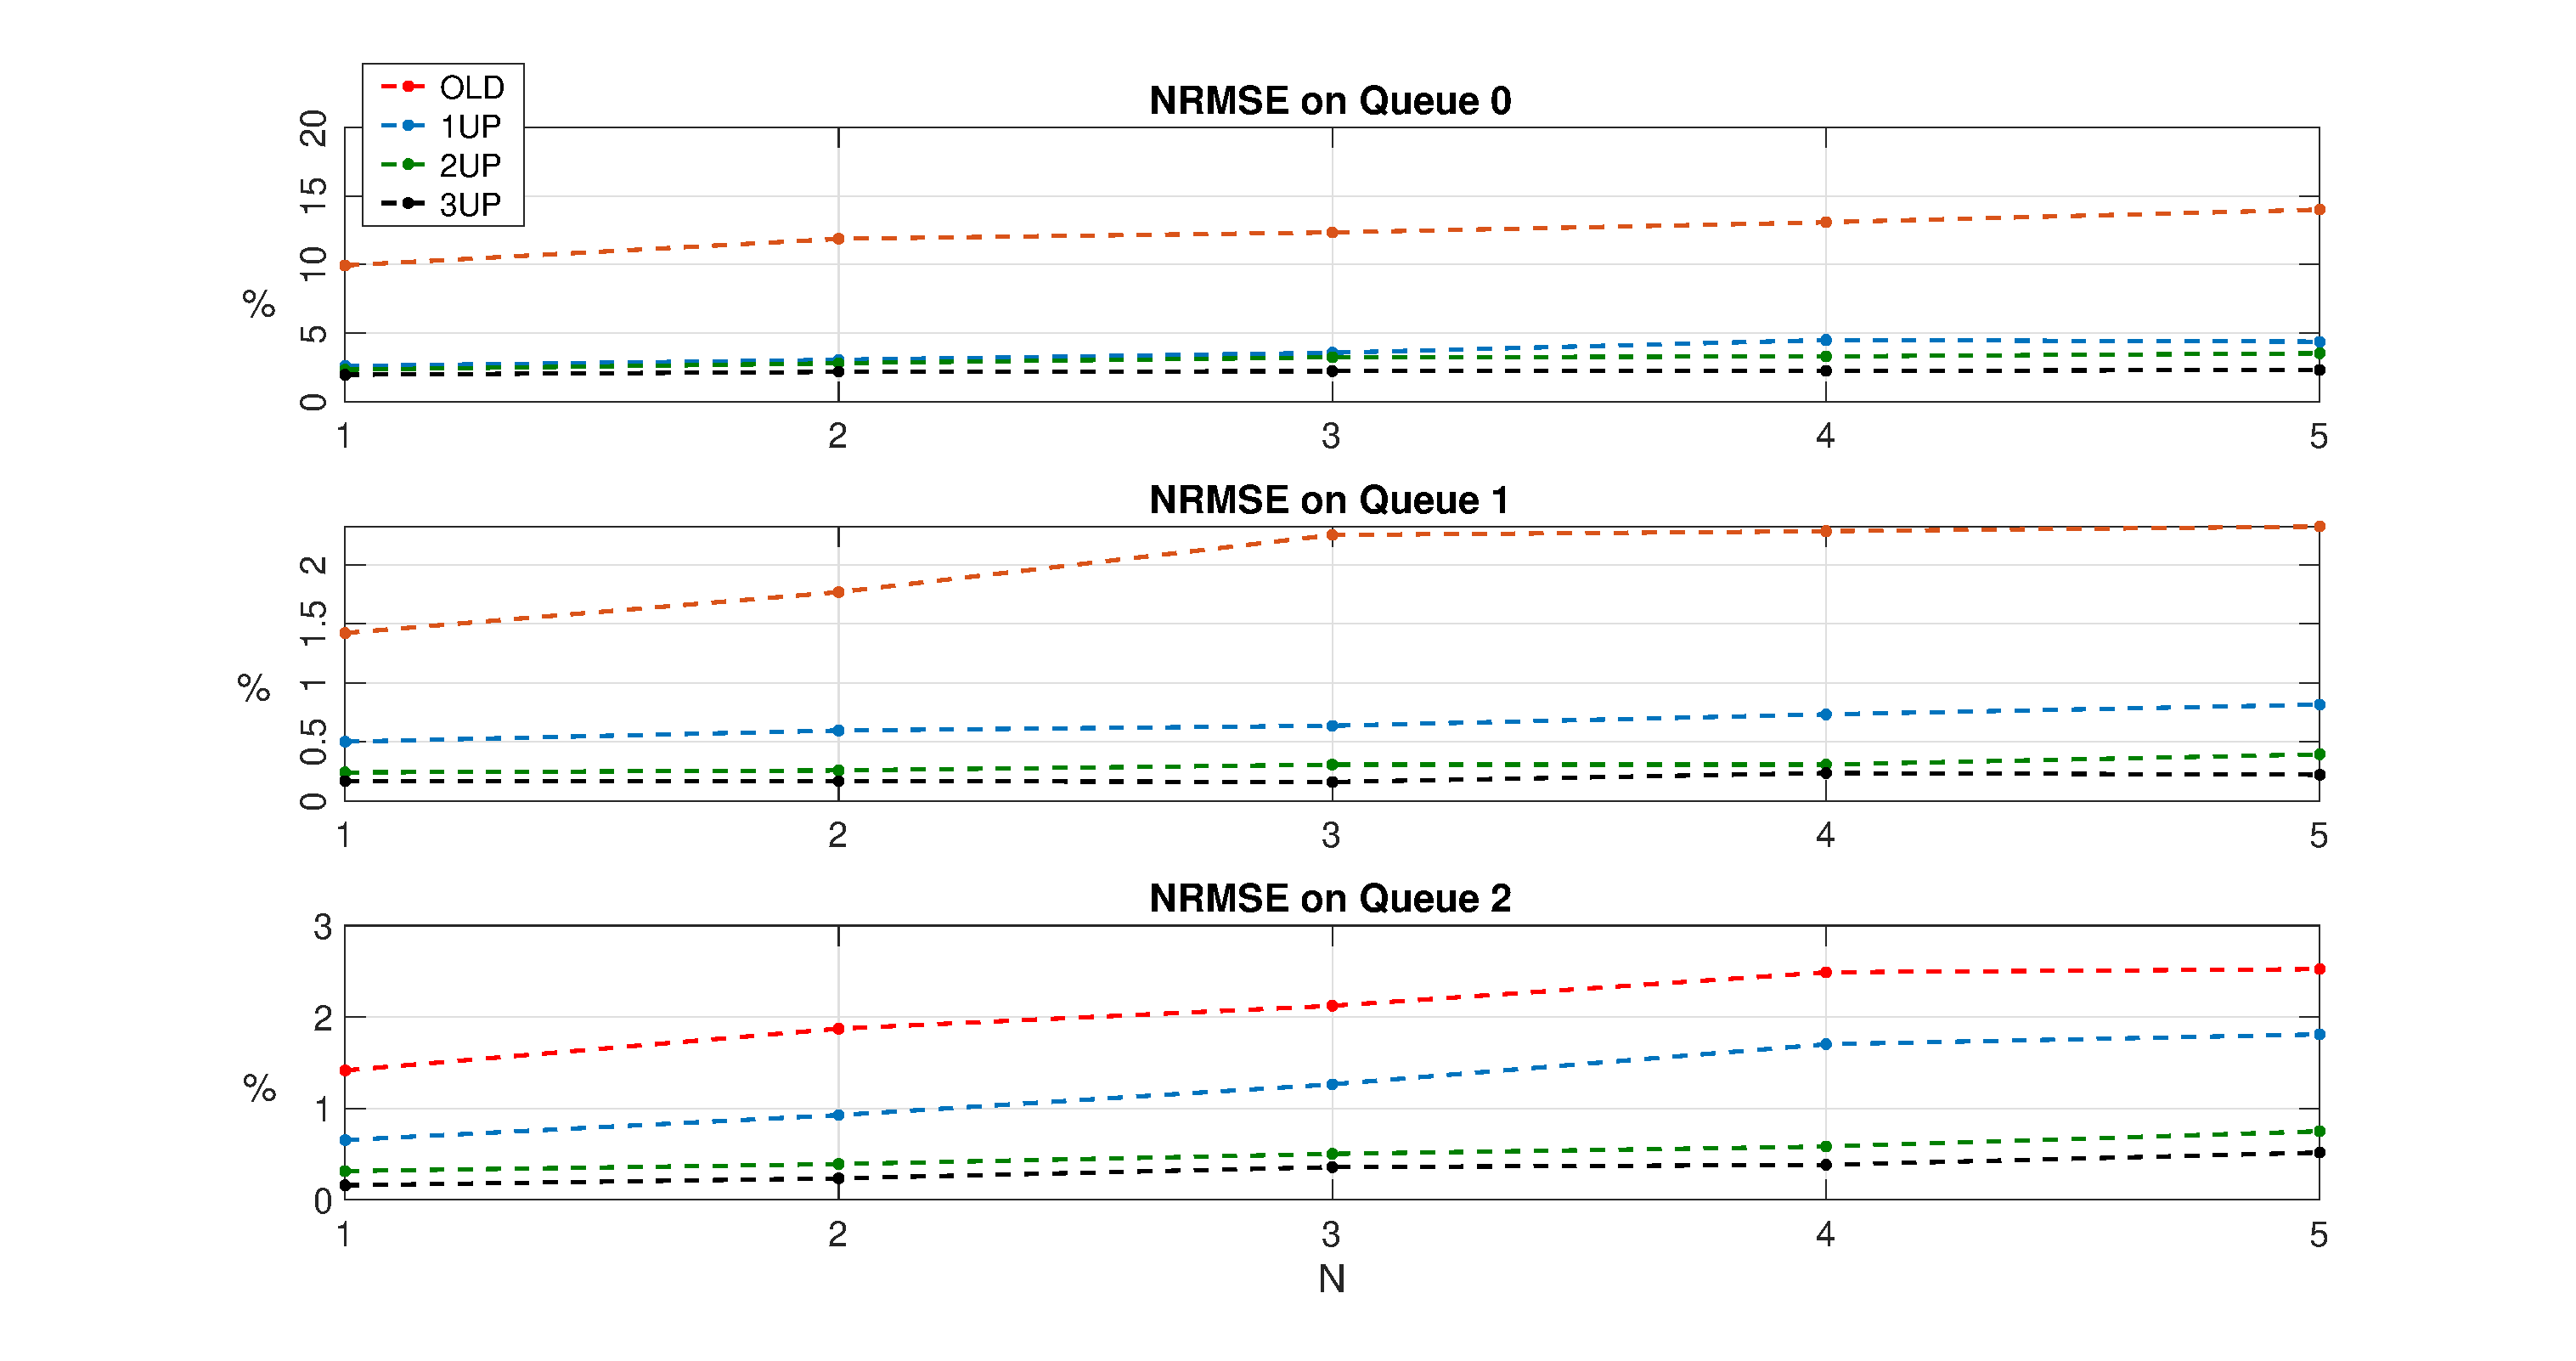
\includegraphics[trim={120 0 120 0}, width=0.9\linewidth]{figure/Error_State_ddM4.eps}
	\caption{NRMSE of the queues output predictive model over a time horizon of $N=5$, with knowledge of the 4-steps future disturbances}
	\label{fig:{stateNRMSEddM4}}
\end{figure}

Figure \ref{fig:{stateNRMSE}} and Figure \ref{fig:{stateNRMSEddM4}} plot the NRMSEs respectively without and with knowledge of the future disturbances. The assumption of future disturbance forecast, as expected, provides much better prediction accuracy. The positive effect of updated data sets is also clear, providing accuracy improvements up to $50 \%$: as will be also discussed in the next section, the most relevant prediction accuracy improvement takes place moving from OLD to 1UP or from 1UP to 2UP, while the 3UP model does not improve much.

\begin{remark}
We wish to highlight that in our simulations we generated data without major modifications of the traffic daily pattern: for this reason enriching the data set converges to a saturation of the model accuracy, as discussed above. Nevertheless, the capability of our methodology to iteratively learn from new data is fundamental as, in real life, changes in the traffic patterns do occur, and model updates are necessary to maintain the model accuracy and the control performance. 
\end{remark}

%====================================================================================================

\subsection{Control performance}

In this section we setup a control loop where the (Mininet) network emulator and the (Ryu) controller run in two different computers, and synchronize/exchange data using a shared file. Namely, our SW controller module is, in principle, ready to be directly used on a real SDN-based network, with just some minor modifications in the data exchange with the switch devices. The controller implements MPC using the predictive models validated in the previous sections: at each time step, it solves Problem \ref{pbMPC} and optimally updates the bandwidth of the different queues. The cost matrices $Q$ and $R$ of Problem \ref{pbMPC} respectively weight the output $y(k)$ of the system (i.e. the packet transmission rate for each queue) and the control input $u(k)$ (i.e. the bandwidth assigned to each queue). Since $R$ is required to be positive definite but it makes no sense assigning a penalty to the choice of $u(k)$, we define $R=10^{-5} \cdot \mathbb I$, where the identity matrix $\mathbb I$ multiplies a very small value. Matrix $Q = diag(1,10^4,10)$ has been assigned as a diagonal matrix, where the choice of the different diagonal components is related to the priority level of each queue. The remaining constraints of Problem \ref{pbMPC} are reported in Table \ref{tab:contPar}.
%The parameters used in the constraints described in Problem \ref{pbMPC} are reported in Table \ref{tab:contPar} and the weights matrices considered in the optimisation cost are: $Q=diag([1,1000,10])$ and $R=10^{-5} \mathbb{I}_3$.
\begin{table}[h!]
	\caption{Constraints in Problem \ref{pbMPC}}
	\centering
	\begin{tabular}{l c l c}
		\hline\hline
		Parameters                                & Value               & Parameters                 & Values       \\ 
		\hline
		$\Delta u_1^\mathrm{min}$     & 1                   & $\Delta u_1^\mathrm{max}$  & 30           \\
		$\Delta u_2^\mathrm{min}$     & 20                  & $\Delta u_2^\mathrm{max}$  & 30           \\
		$\Delta u_3^\mathrm{min}$     & 20                  & $\Delta u_3^\mathrm{max}$  & 20           \\
		$u_1^\mathrm{min} $             & 10                  & $u_1^\mathrm{max} $        & 45           \\
		$u_2^\mathrm{min} $            & 55                  & $u_2^\mathrm{max} $        & 80           \\
		$u_3^\mathrm{min} $            & 80                  & $u_3^\mathrm{max} $        & 100          \\
		
		\hline
	\end{tabular}
	\label{tab:contPar}
\end{table}
In what follows we validate the control performance both without and with knowledge of the future disturbances. The value of $x_\mathrm{ref}$ in the optimization problem represents the reference value we chose for tracking system output: indeed, as we wish to minimize packet losses, we minimize the difference between the packets received by the hosts $d(k)$ and those transmitted by the queues $y(k)$ over the horizon $N$. In case we have no knowledge of future disturbances, we consider $x_\mathrm{ref}$ equal to the current disturbance  measurement $d(k)$ and constant over all the predictive horizon; if instead we have knowledge of future disturbances, we consider $x_\mathrm{ref}$ equal to such future disturbances. In this section we decided to only compare models OLD, 1UP and 2UP, since model 3UP does not provide any substantial improvement. 

 \begin{figure}[h!]
	\centering
	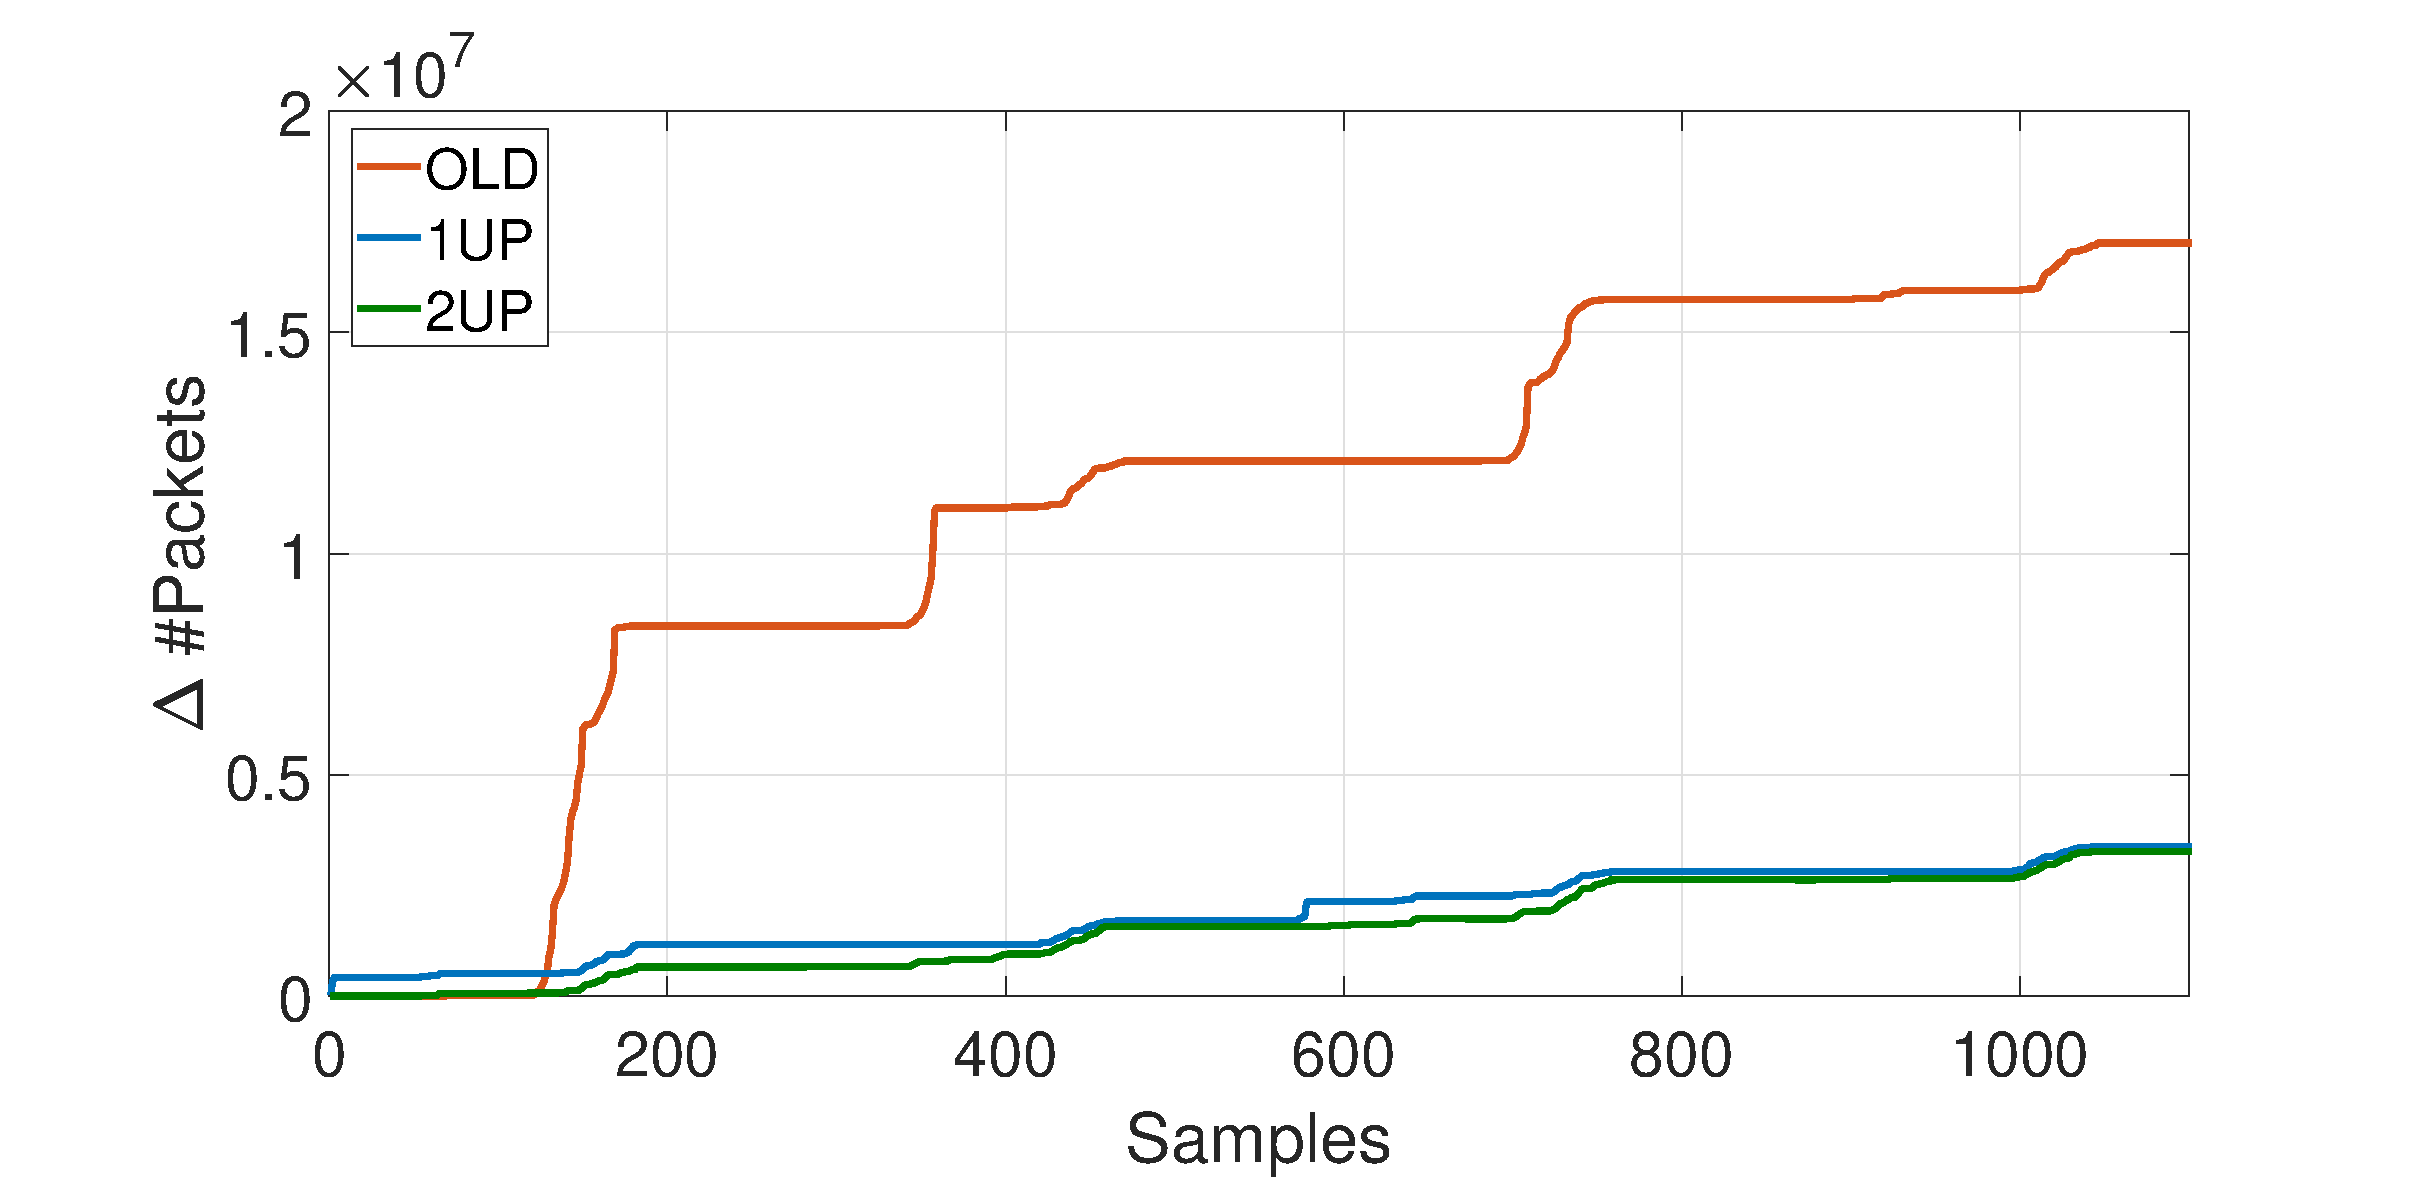
\includegraphics[trim={120 0 120 0}, width=0.9\linewidth]{figure/cumPL1.eps}
	\caption{Cumulative Packet Losses without knowledge of the future disturbance.}
	\label{fig:{MPC1}}
\end{figure}
\begin{figure}[h!]
	\centering
	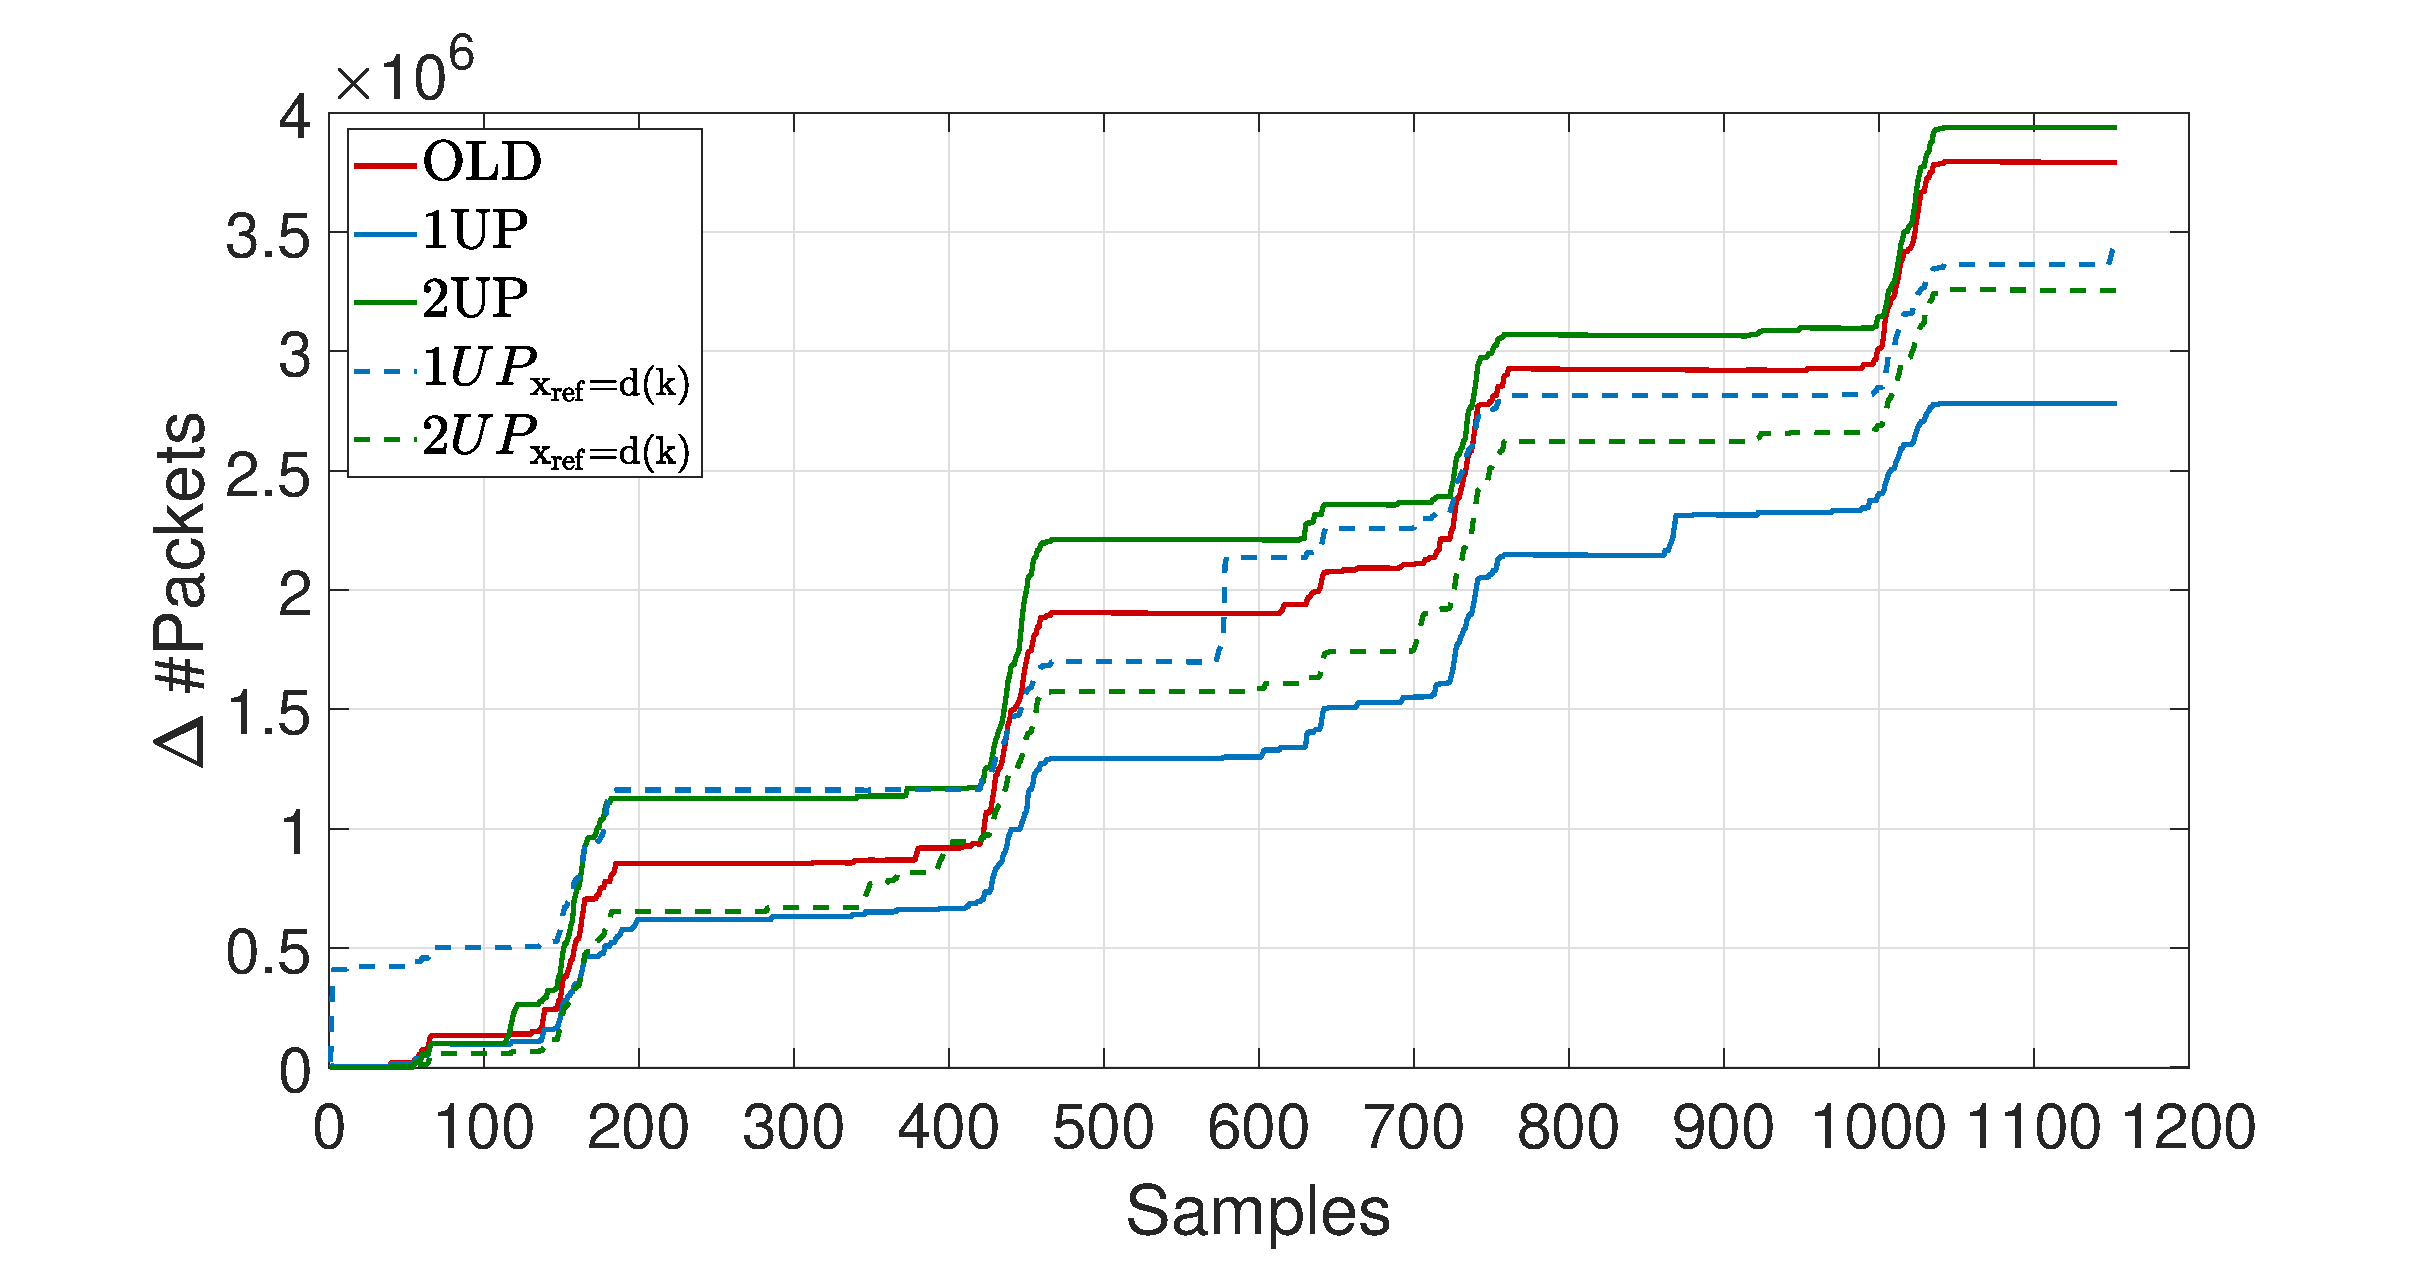
\includegraphics[trim={120 0 120 0},width=0.9\linewidth]{figure/cumPL_Total.eps}
	\caption{Comparison between Cumulative Packet Losses with (solid lines)  and without (dashed lines) knowledge of the future disturbance.}
	\label{fig:{MPC2}}
\end{figure}
 Figures \ref{fig:{MPC1}} and \ref{fig:{MPC2}} plot the cumulative packet losses respectively without and with knowledge of the future disturbances. The packet loss rate when the control is performed exploiting the OLD model and without disturbance forecast is around $123\%$ larger than all other cases (and, of course, incomparably smaller than the static control case \cite{Notiziario}). It is also clear from the plots that 1UP and 2UP without disturbance forecast and OLD, 1UP and 2UP with disturbance forecast provide very similar performance. Our interpretation is that OLD models without disturbance forecast have not enough information to provide good accuracy, but they can be easily improved either with a data set update (which however requires $10$ days for 1UP and $20$ days for 2UP of additional data) or using a predictive disturbance model.

\begin{figure}[h!]
\centering
\subfigure[a][]{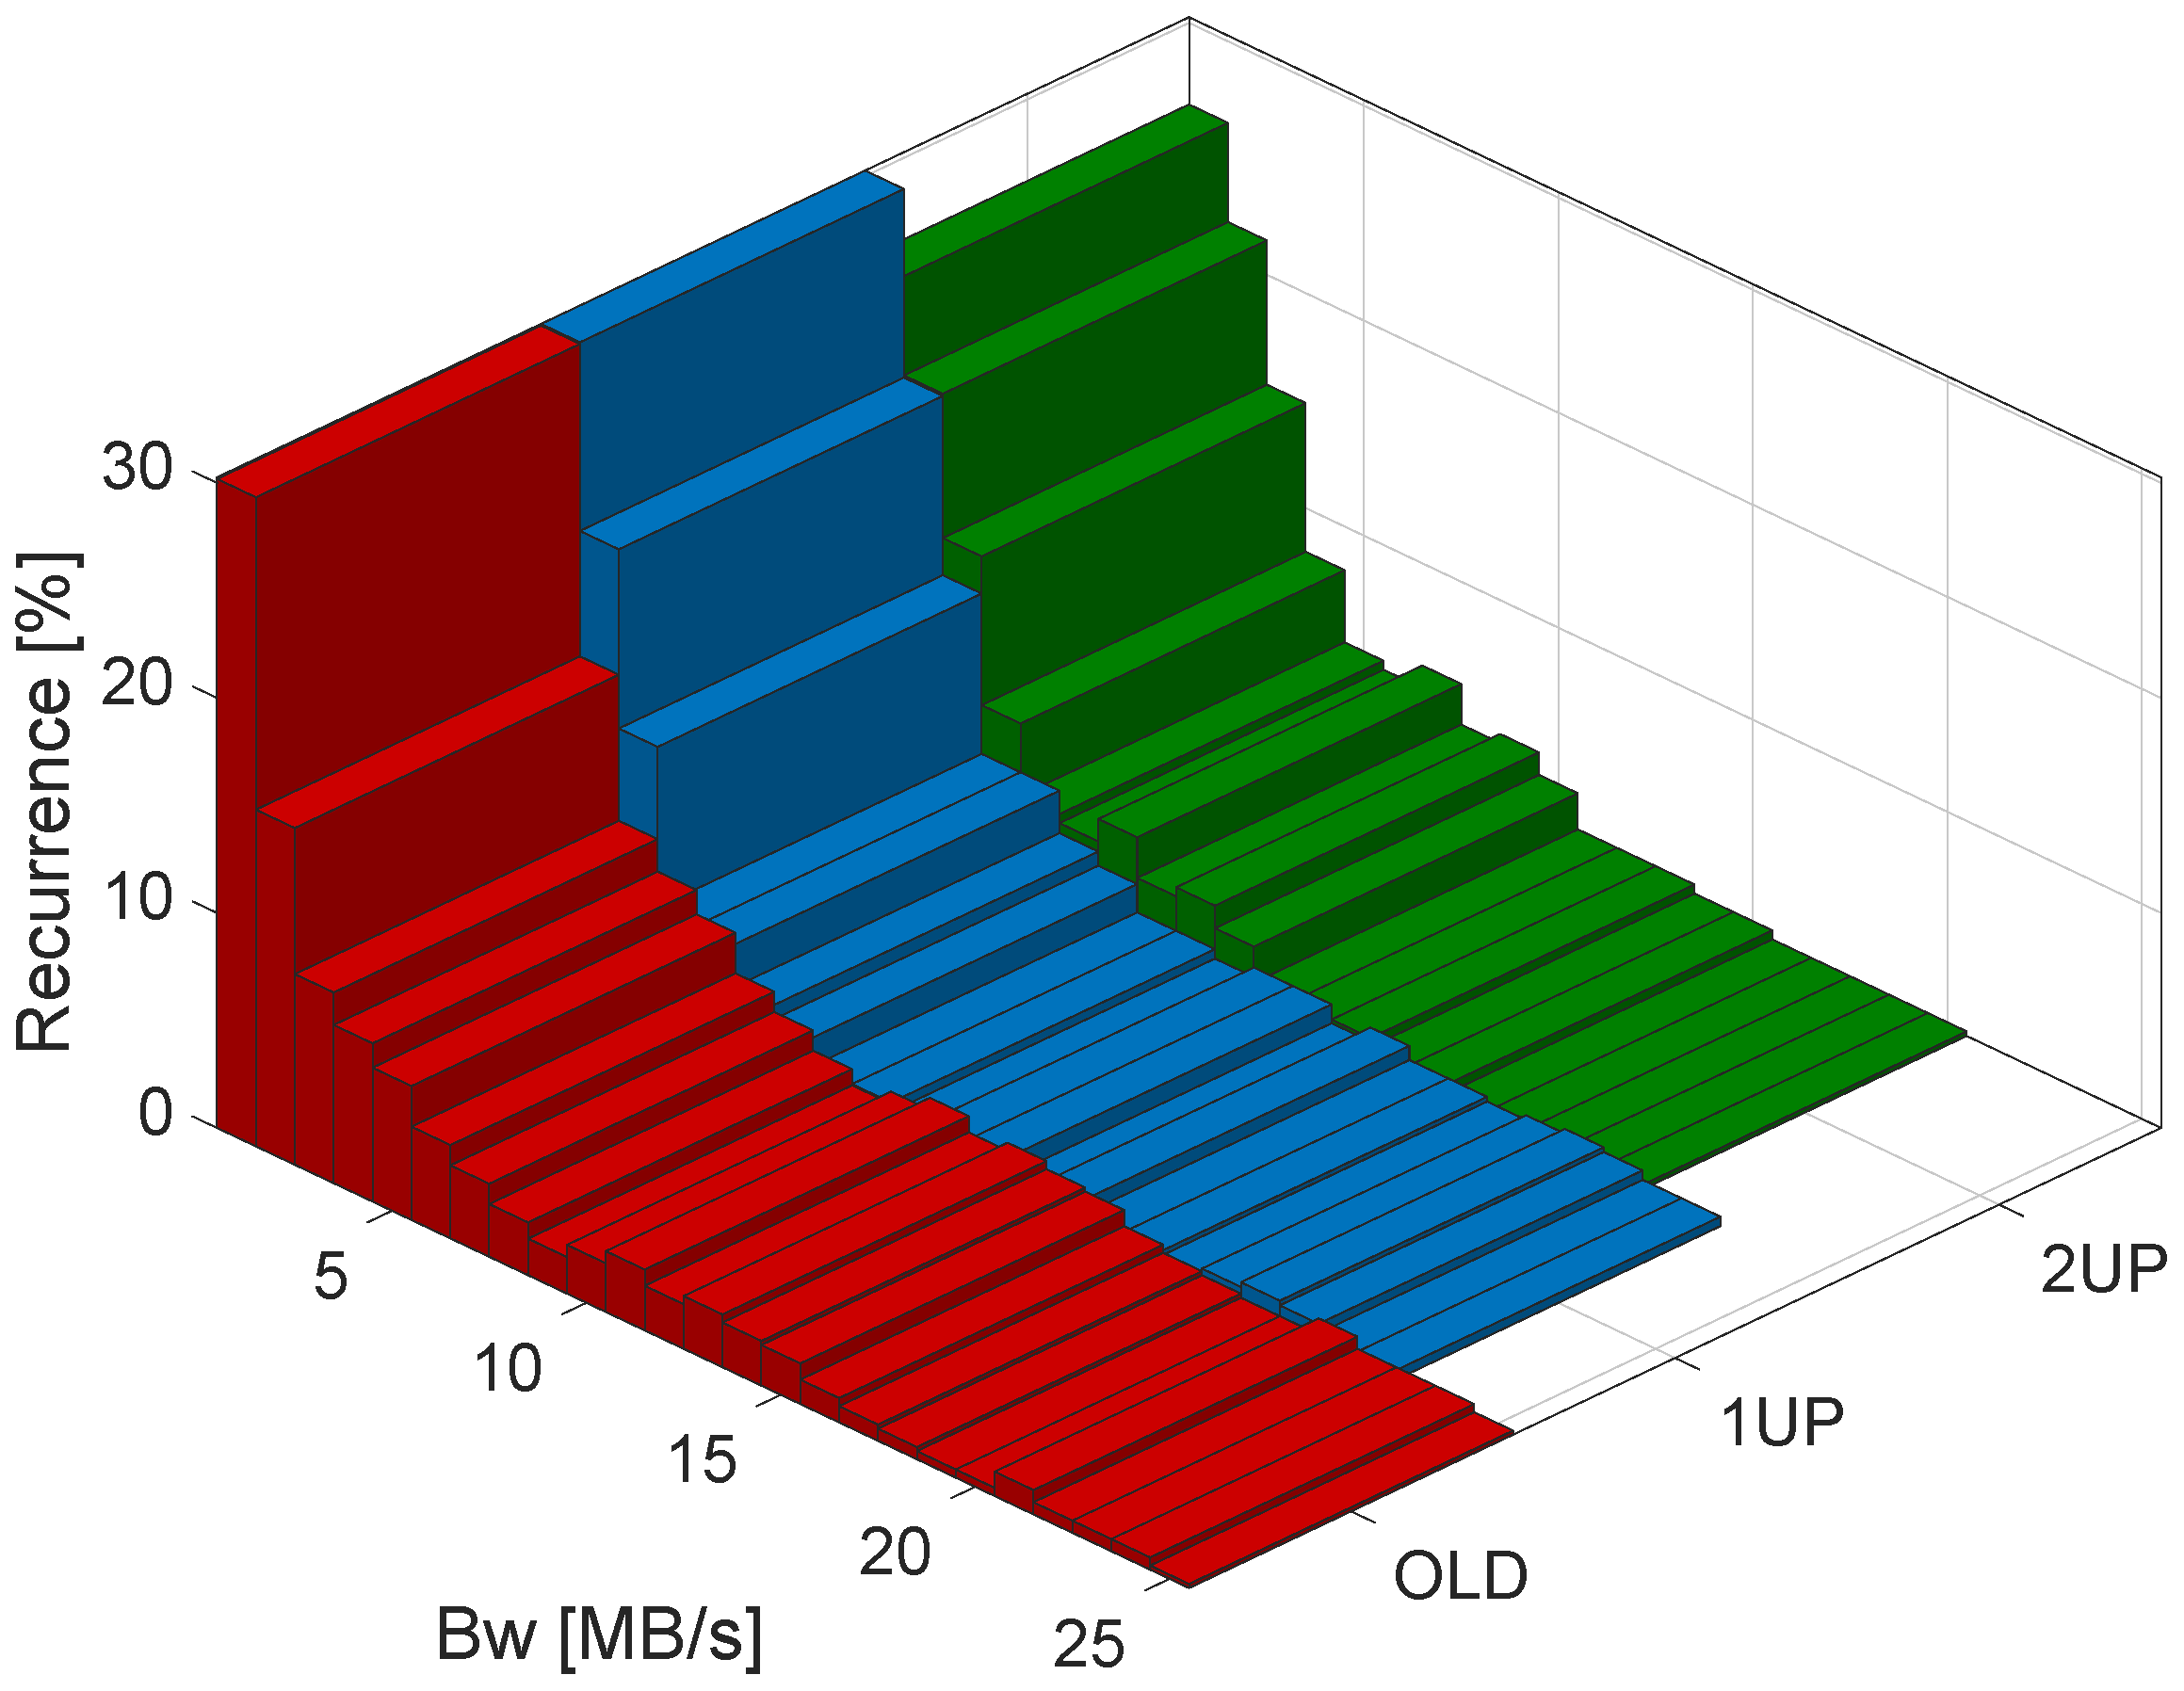
\includegraphics[width=0.7\linewidth]{figure/BW_NoPred.eps}}
\subfigure[b][]{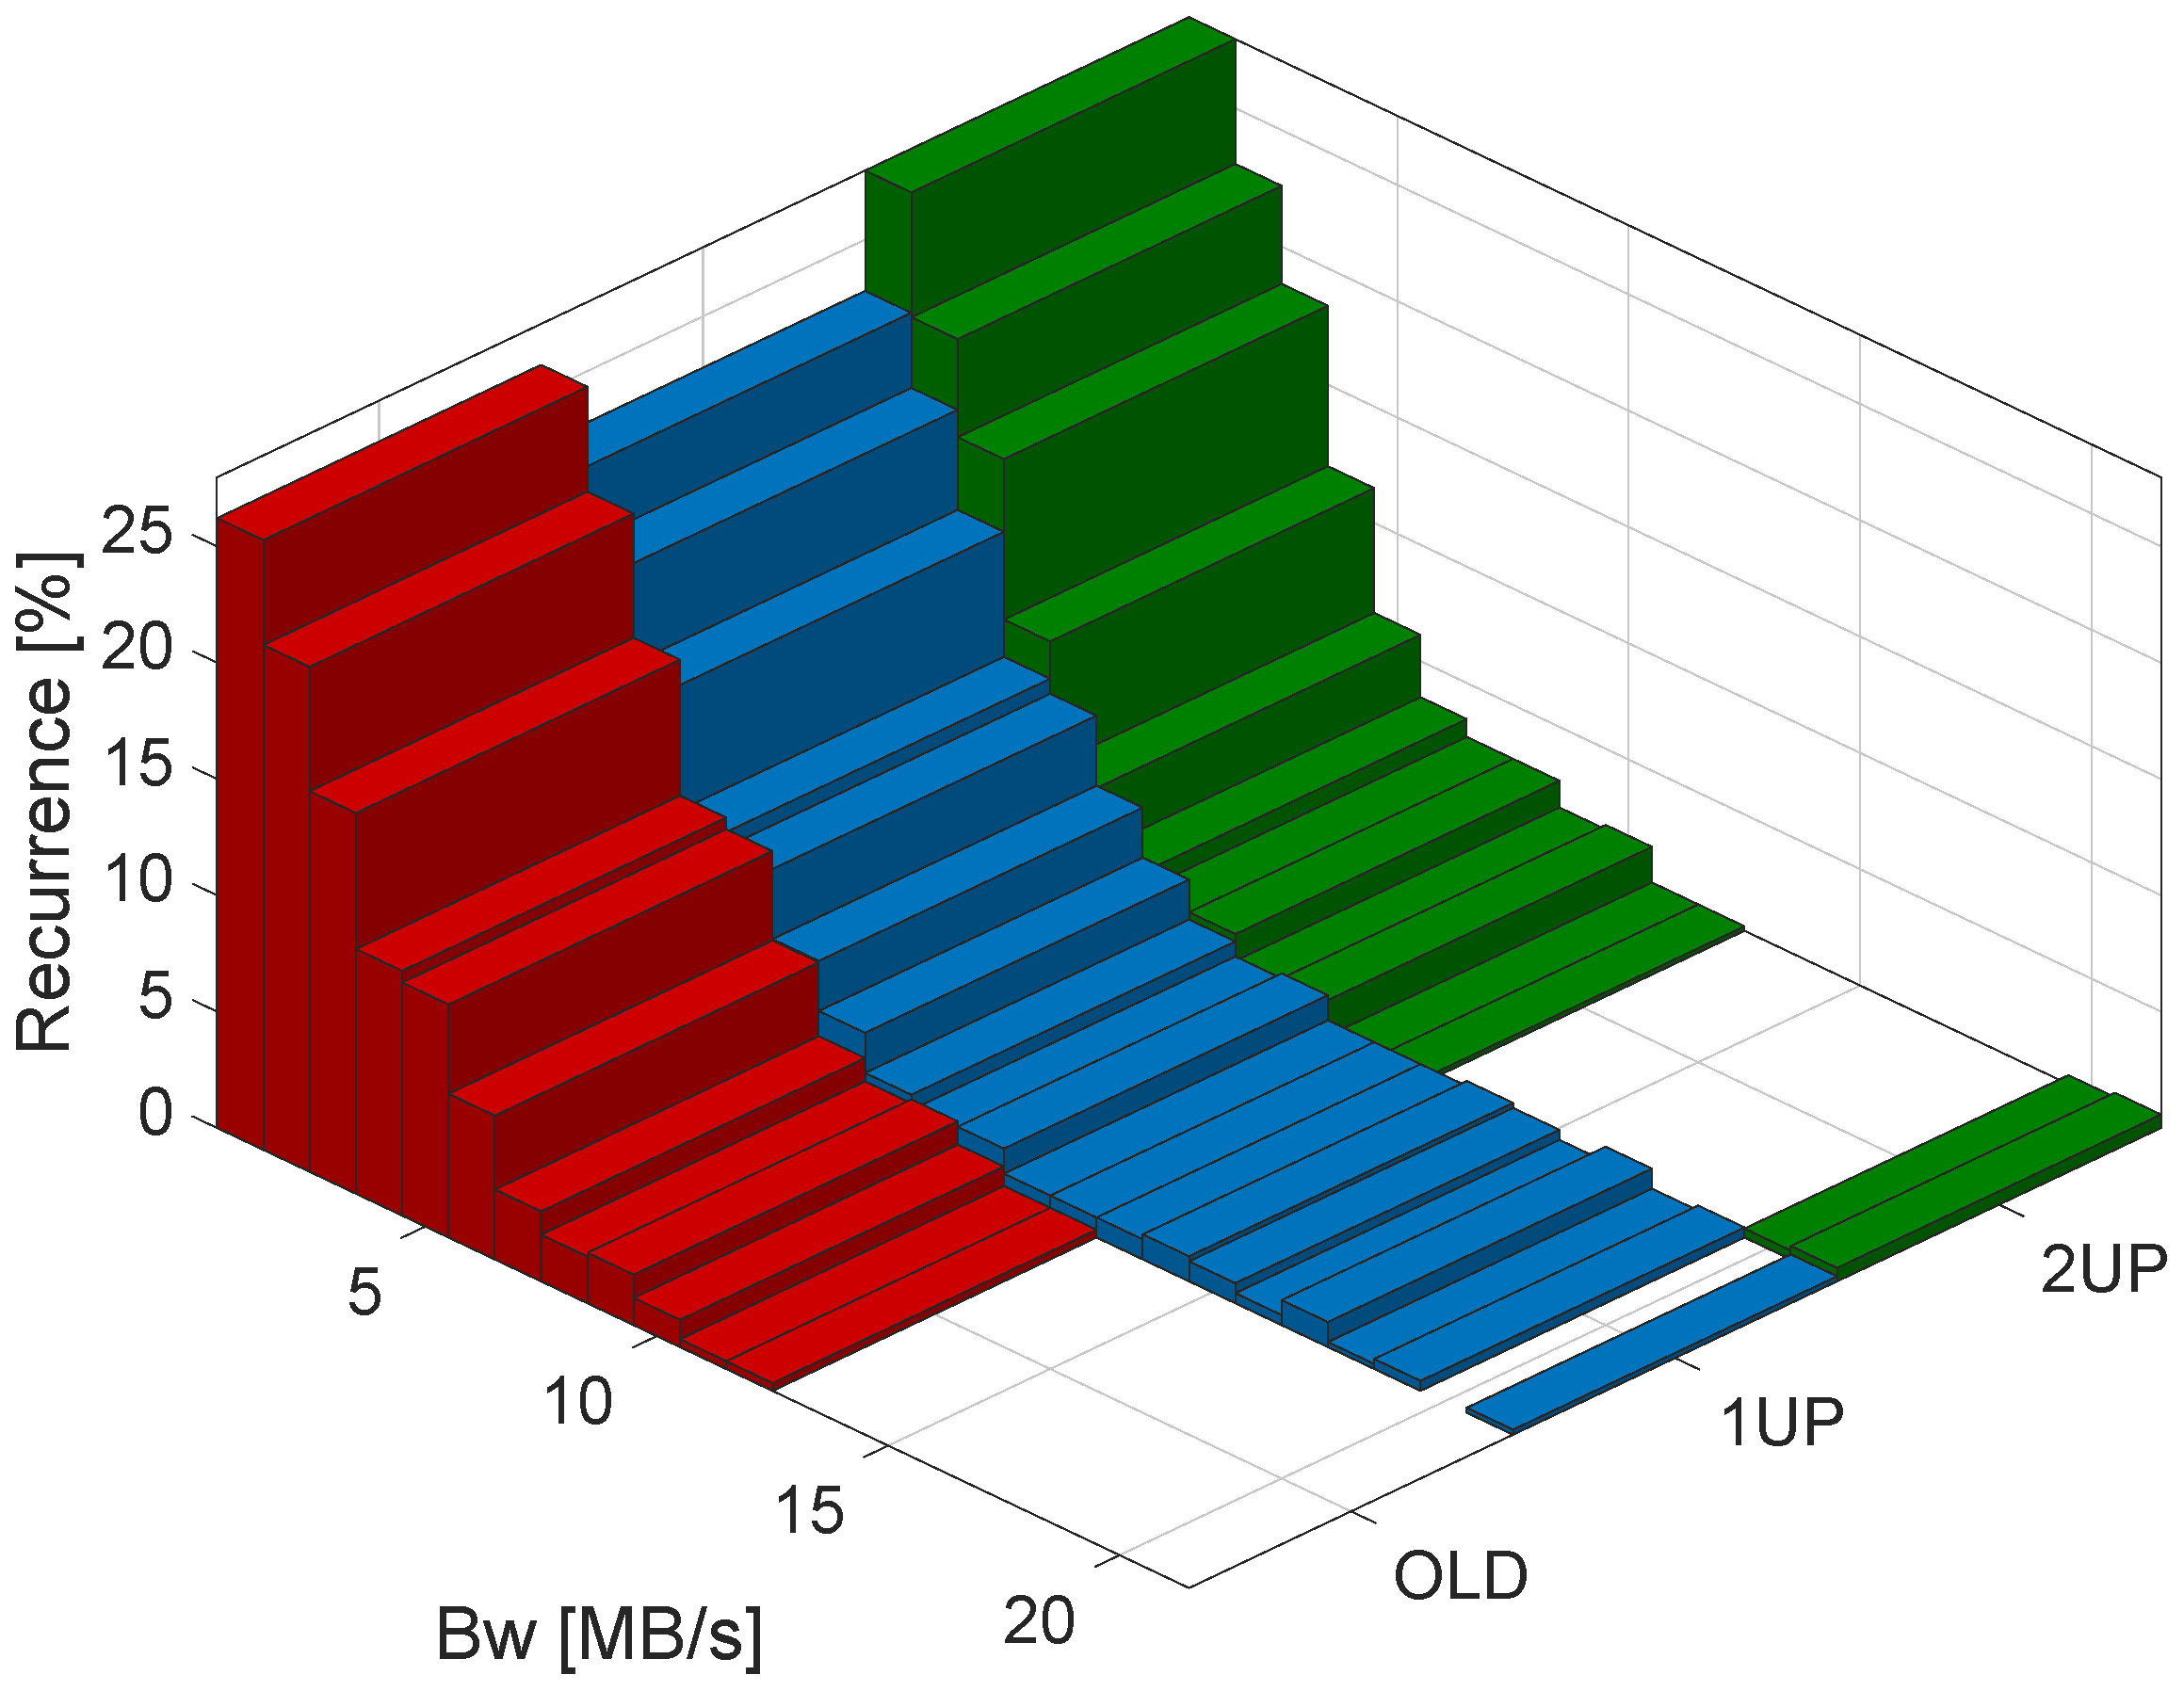
\includegraphics[width=0.7\linewidth]{figure/BW_Pred.eps}}
\caption{Bandwidth saving comparison without (a) and with (b) knowledge of the future disturbances.}
\label{fig:BW}
\end{figure}

Figure \ref{fig:BW} illustrates the bandwidth savings showing the recurrence of the different bandwidth usage during the simulations, respectively without and with knowledge of the future disturbances. Without disturbance forecast we exploited up to $25MB/s$ using the OLD model, while we exploited at most $22MB/s$ and $21MB/s$ respectively for models 1UP and 2UP. Using disturbance forecast, as expected, even less bandwidth is exploited.

\begin{figure}[h!]
\centering
\includegraphics[trim={120 0 120 0},width=0.9\linewidth]{figure/MPCfinal.eps}
\caption{Static controller up to the $400th$, then MPC controller.}
\label{fig:{MPC}}
\end{figure}
%\begin{figure}[h!]
%	\centering
%	\includegraphics[trim={120 0 120 0},width=0.7\linewidth]{figure/banda.eps}
%	\vspace{-0.2cm}
%	\caption{MPC controller: packets sent from the queues (orange), packets lost (red), bandwidth saving (blue).}
%	\vspace{-0.5cm}
%	\label{fig:{BWsave}}
%\end{figure}

We conclude this paper by quantifying the gap between priority queueing control performance of MPC, obtained solving Problem \ref{pbMPC} and based on our RF predictive model, with the static control policy adopted by service provider networks in \cite{Notiziario}. Figure \ref{fig:{MPC}} highlights the dramatic improvement of MPC with respect to static control: the red line shows the incoming traffic, the blue line shows the sum of the packets sent from the queues, and their difference represents packet losses. Until the $400th$ static control has been implemented as in \cite{Notiziario}, generating many packet losses due to queues saturation. From that sample to the end of our experimentation we implemented MPC using our RF-based model, drastically reducing packet losses: quantitatively, after $700$ sampling periods the cumulative number of dropped packets with the static policy is about $5.5\cdot10^8$ versus $6.6\cdot10^6$ with MPC, with a decrease of $5.434\cdot10^8$ lost packets ($-88 \%$).
%Figure \ref{fig:{BWsave}} shows the amount of bandwidth that our method leaves unused at each time sample (blue line): during the simulation period we were able to save an average $3 MB/s$ with respect to static control, with peaks of more than $20 MB/s$, that can be of course allocated to improve the quality of other services.
We remark that, even thought the improvement of MPC with respect to static control is not surprising, much better performance can be obtained in real networks just collecting historical data and applying a controller that can be directly implemented using the accurate models of our identification algorithms and Quadratic Programming standard solvers.